\documentclass[a4paper]{report}
%\usepackage[textwidth=18cm,textheight=23cm]{geometry}
%\usepackage[textwidth=15.5cm,textheight=23cm]{geometry}
\usepackage{geometry}
\usepackage[square]{natbib}
\usepackage[usenames,dvipsnames]{color}
\usepackage{listings}
\usepackage{float}
\usepackage{graphicx}
\usepackage{caption}
\usepackage{enumerate}
\usepackage{parskip}
\usepackage{amsmath}
\usepackage{pdfpages}
\linespread{1.5}

%\setlength{\hoffset}{0.49606in}
%\setlength{\hoffset}{1.26cm}
\geometry{left=3.8cm, bottom=2cm, top=2cm, right=2cm}

\definecolor{lightlightgray}{gray}{0.9}

\newcommand{\modulo}{ \, \textbf{mod} \, }
\newcommand{\bigo}[1]{ \mathcal{O} (#1)}
\newcommand{\degree}{\ensuremath{^\circ}}

\newcommand{\lstAlgo} {
	\lstset{
		language=C,
		backgroundcolor=\color{white},
		basicstyle=\small,
		keywordstyle=\color{blue},
		commentstyle=\color{OliveGreen},
		stringstyle=\color{red},
		tabsize=4,
		captionpos=t,
		title=\lstname,
		frame=single,
		lineskip={-0.3pt},
		morekeywords={endif, then, call, func, endfunc, proc, endproc, foreach, endfor, endwhile, AND, OR, NOR, XOR}
	}
}
\newcommand{\lstCpp}{
	\lstset{
		language=C++,
		backgroundcolor=\color{lightlightgray},
		basicstyle=\ttfamily\scriptsize,
		keywordstyle=\color{blue},
		commentstyle=\color{OliveGreen},
		stringstyle=\color{red},
		tabsize=4,
		captionpos=t,
		title=\lstname,
		frame=single,
		lineskip={-0.3pt},
		breaklines=true
	}
}

%\newcommand{\lstcodewd}[1]{\hspace{4ex} \frame{\footnotesize\emph{#1}}}

\begin{document}
% Old cover page
%\title{\textbf{CMPMP2Y --- MSc Dissertation: \\ Procedural Generation of Dungeons}}
%\author{Olivier Legat \\ (Supervisor: Prof. Andy Day)}
%\maketitle

% New cover page
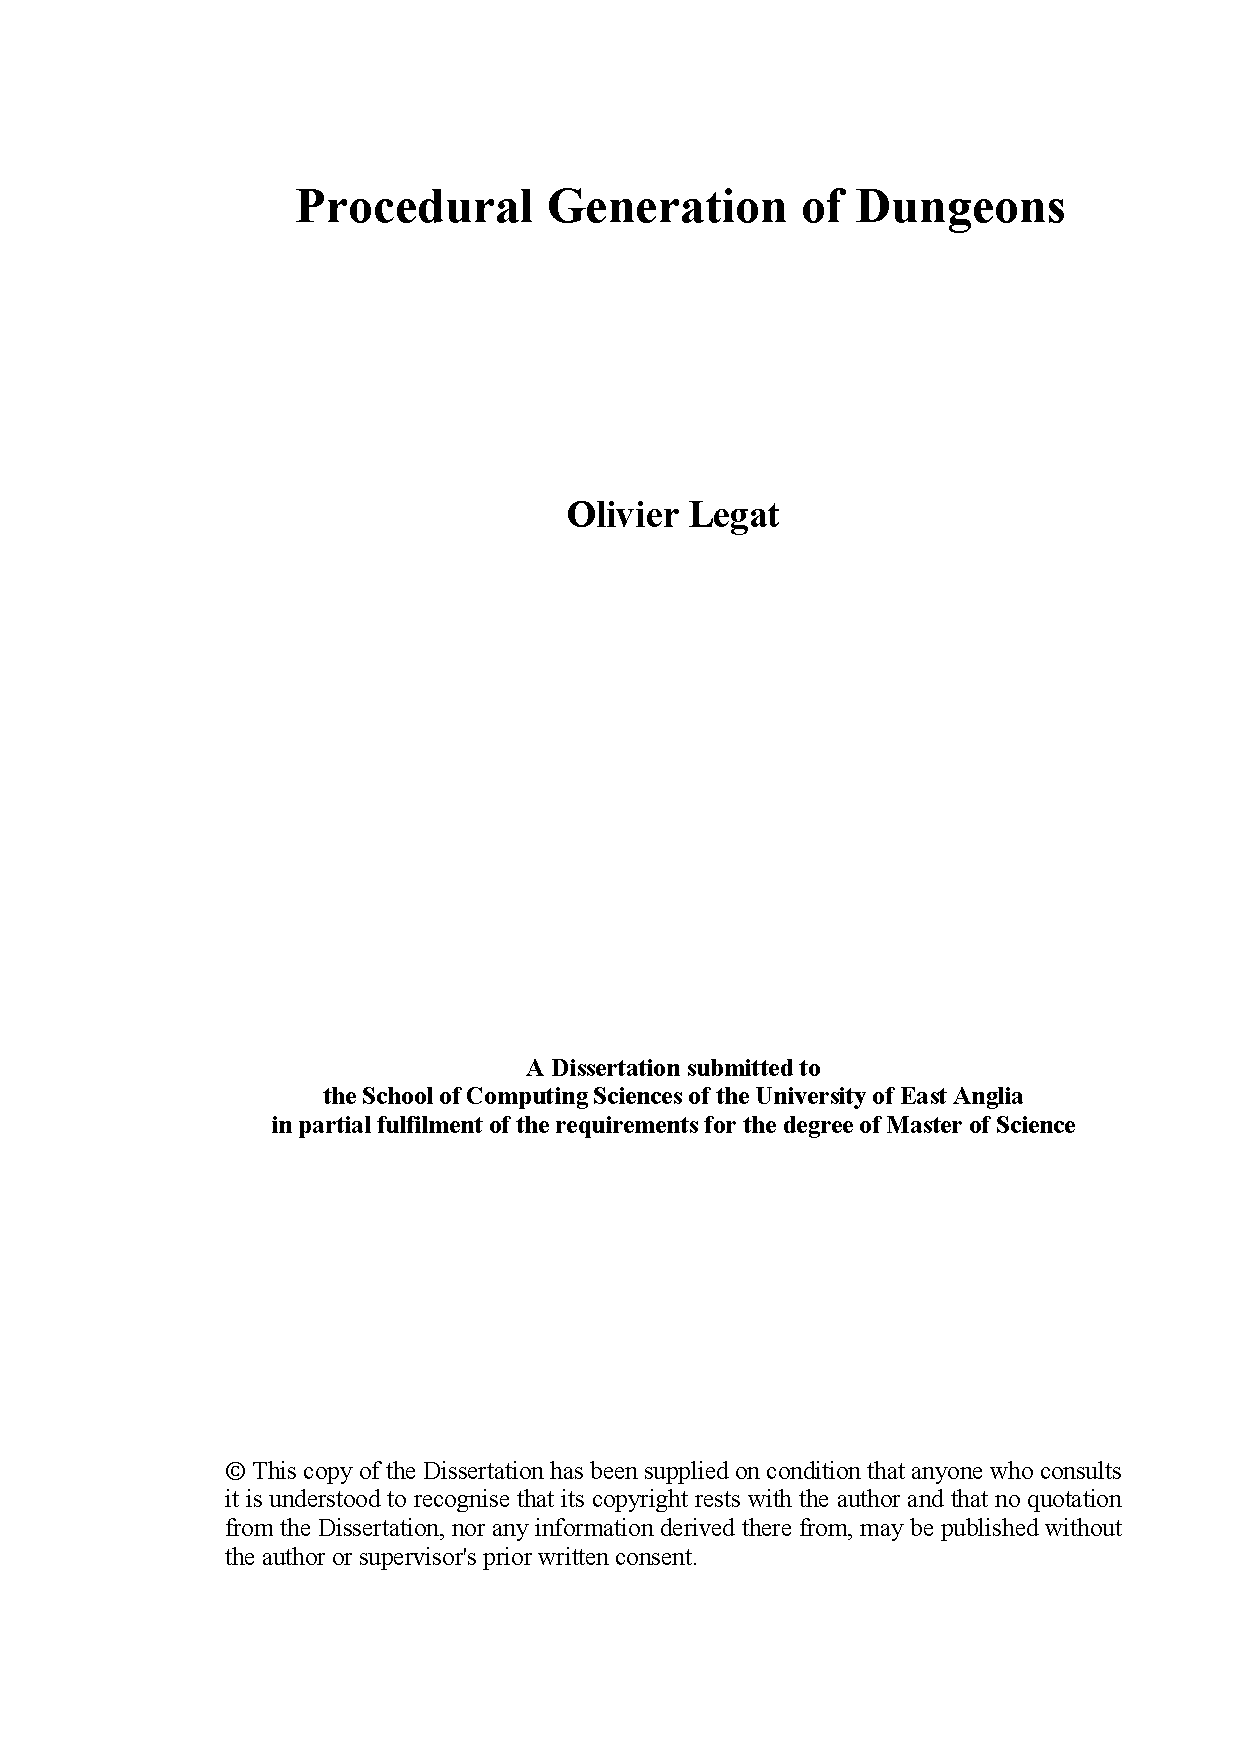
\includepdf[pages=1]{CoverSheet.pdf}

\begin{abstract}
The use of procedural content generation (PCG) is not un-common amongst games, it appears in many applications. PCG algorithms notably present the advantage of providing potentially infinite and un-predictable content for the players, which can significantly add value to the game. However, implementing a good PCG algorithm that generates convincing results is not a trivial task. PCG revolves around the concept of randomness that is usually implemented by using pseudo-random number generators. Different PCG methods can be used to create content for specific kinds of environments. These methods can vary greatly depending on the type of environment desired. This thesis focuses on generating content for dungeon-like or maze-like environments by identifying the most suitable methods and algorithms. The methods used for generating maze involve finding a random spanning tree of a graph, hence the Prim's and Kruskal's algorithms can be used. Further on, we can obtain a dungeon-like environment from a maze by applying modifications to it such as adding loops and rooms.
\end{abstract}

\setcounter{page}{1}
\pagenumbering{roman}

\pagebreak
\chapter*{Acknowledgement}
\begin{quotation}
This dissertation would have never been completed if not for the help of several people who offered their services and help to me.
\end{quotation}
\begin{quotation}
First and foremost, I would like to thank my parents, Thierry and Carol whom I hold dearly to me, for their love, their financial and moral support, and for never losing faith in me throughout the year despite the circumstances.
\end{quotation}
\begin{quotation}
I would like to express my deepest gratitude to my supervisor Professor Andy Day for accepting my self-proposed topic without a second doubt and later providing his advice, guidance and feedback on my progress.
\end{quotation}
\begin{quotation}
I would also like the thank Dr. Wenjia Wang, the MSc Dissertation Module organiser, who has taught me how to write a proper MSc thesis. His help was a valuable asset to completing my work on time. 
\end{quotation}
\begin{quotation}
I want to thank Dr. Rudy Lapeer and Dr Stephen Laycock for teaching me all there is to know about Graphics, Rendering and Real-time Virtual Environments.
\end{quotation}
\begin{quotation}
I send my humble thanks to Abiishiek Vijaykumar for spending many hours thoroughly proof-reading my entire dissertation. Without his help this write-up would have certainly not met to the standard of a MSc Dissertation.
\end{quotation}
\begin{quotation}
I would like to thank all my fellow friends in Norwich whom have stood with me through the tough times, helped me in every way they could and given me the strength to keep going.
\end{quotation}

% Table of Contents Page(s)
\pagebreak
\tableofcontents
\pagebreak

\setcounter{page}{1}
\pagenumbering{arabic}

\chapter{Introduction}

	\section{What is PCG?}
Level design is a crucial factor in video games that has been around for as long as games have. It consists of manually designing an environment by specifically defining every bit of detail and importing them directly into the game. Such details include, but are not limited to: Terrain shape, goals or mission objectives, location of enemies and collectible objects. This is called {\em level designing}, and it's traditionally done by a human-being known as an {\em artist} or {\em game designer}.

However, level designing is not the only method to create the virtual environment of a video game. Another method is to procedurally generate a virtual environment. The concept behind this method is to write an algorithm that will design a level by using randomly generated numbers as opposed to leaving the task to a human. This is called {\em level generation}. This can greatly increase the amount of content or the value of a game. For this reason, it is not uncommon for games to include this method. Naturally, this procedural method differs greatly from traditional level designing that is more directed towards an artistic path.

Procedural Content Generation (PCG) is the general term used to describe the creation of any random computer-designed objects within a game. PCG can refer to the creation of any kind of randomised object, such as non-playable characters (NPCs), the weapons they can use, and so forth. Although generally speaking, PCG refers to the generation of the game's environment, such as creating a randomised mountain terrain or maze for example.

In the course of this dissertation, the focus will be targeted towards the creation of the environment itself, more specifically, to creation of a maze or a dungeon.

	\section{A short history}
Level generation is not particularly a new concept. It has been around for a significant amount of time and has been implemented in a number of games.

	\subsection{Rogue-like games}

With regards to dungeon-generation, the most popular example is probably {\em Rogue}, a game created in the 1980s \citep{DBLP:journals/tciaig/AshlockLM11}. This game was the first of its kind and was evidently a big success. Later on, many games like {\em Diablo}, {\em NetHack}, {\em Moria} and {\em Dwarf Fortress} \citep{DBLP:conf/cig/TogeliusPBWHY10} followed the same style but improved the features of Rogue. These types of games are generally referred to as {\em rogue-like} games.
\begin{figure}[h!]
\centering
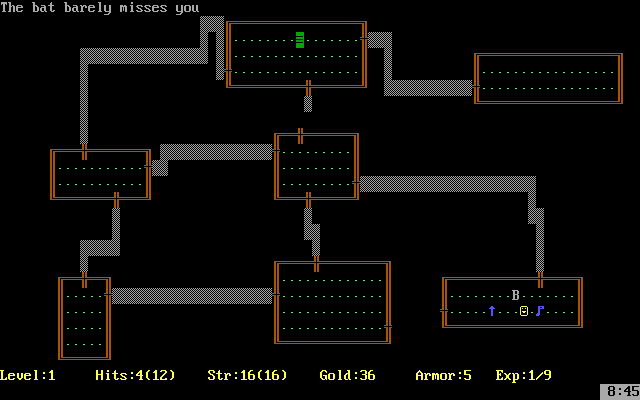
\includegraphics[width=0.50\textwidth]{images/Rogue0.png}
\caption{A screenshot of the console-based game {\em Rogue}.
\\{\footnotesize http://tripalot.com/roguelike/img/rogue.gif} }
\end{figure}

NetHack had improved on Rogue by adding more detail to the dungeons. The game itself would take up about 2 MB of disk space, which at that time was considered a lot. Due to the level of detail in NetHack, it was found to be far less predictable and more enjoyable than Rogue. The amount of content in NetHack is probably what made it so successful \citep{Roguelike}.
\begin{figure}[h!]
\centering
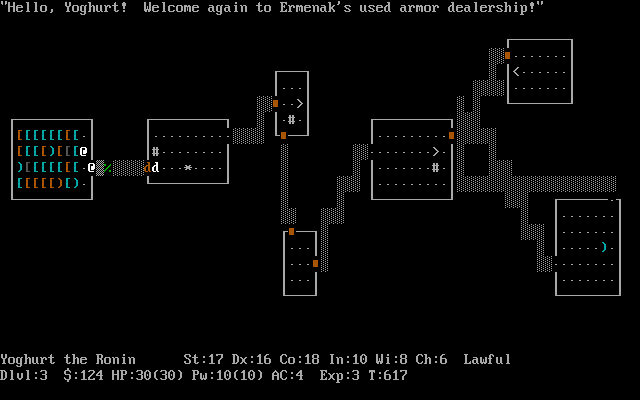
\includegraphics[width=0.50\textwidth]{images/nethack.png}
\caption{{\em HetHack}, a successor of Rogue.
\\{\footnotesize http://tripalot.com/roguelike/img/nethack.gif} }
\end{figure}

Moria also improved upon Rogue by adding an exceedingly large amount of content, even more than NetHack. It had more monsters, more spells, more items and etc., taking this genre of games to the next level \citep{Roguelike}.
\begin{figure}[h!]
\centering
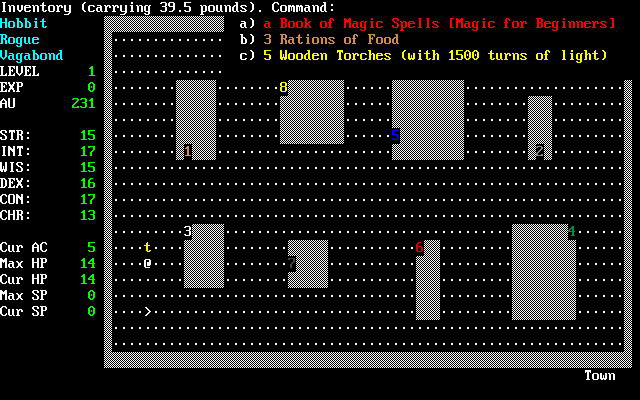
\includegraphics[width=0.50\textwidth]{images/moria.png}
\caption{A screenshot of {\em Moria} (a.k.a. {\em Angband}).
\\{\footnotesize http://tripalot.com/roguelike/img/angband.gif} }
\end{figure}

	\subsection{Other games}
Some games such as Borderlands and Left 4 Dead have pseudo-random levels, meaning that the overall layout of the game's level is designed by hand but contains some randomised features \citep{DBLP:journals/tciaig/TogeliusYSB11}. Other games such as Diablo completely discarded level designing and randomly generated all the levels, NPCs and props \citep{Nitsche-CaseStudy}.

One notable example is Minecraft, a game originally designed by the Swedish developer Markus Persson (a.k.a ``Notch") who later founded the game studio Mojang \footnote{http://www.minecraft.net/game/credits (Date accessed: 28th Feburary)}. In Minecraft, the player is placed in a world composed of different types of blocks. The blocks are placed at random using Perlin noise \footnote{http://pcg.wikidot.com/pcg-games:minecraft (Date accessed: 28th Feburary)}. The wide range of block types allows the player to experience different biomes.  The world is pseudo-infinite; meaning that, as the player moves into unexplored areas, the game will automatically generate more content to fill that area.
\begin{figure}[h!]
\centering
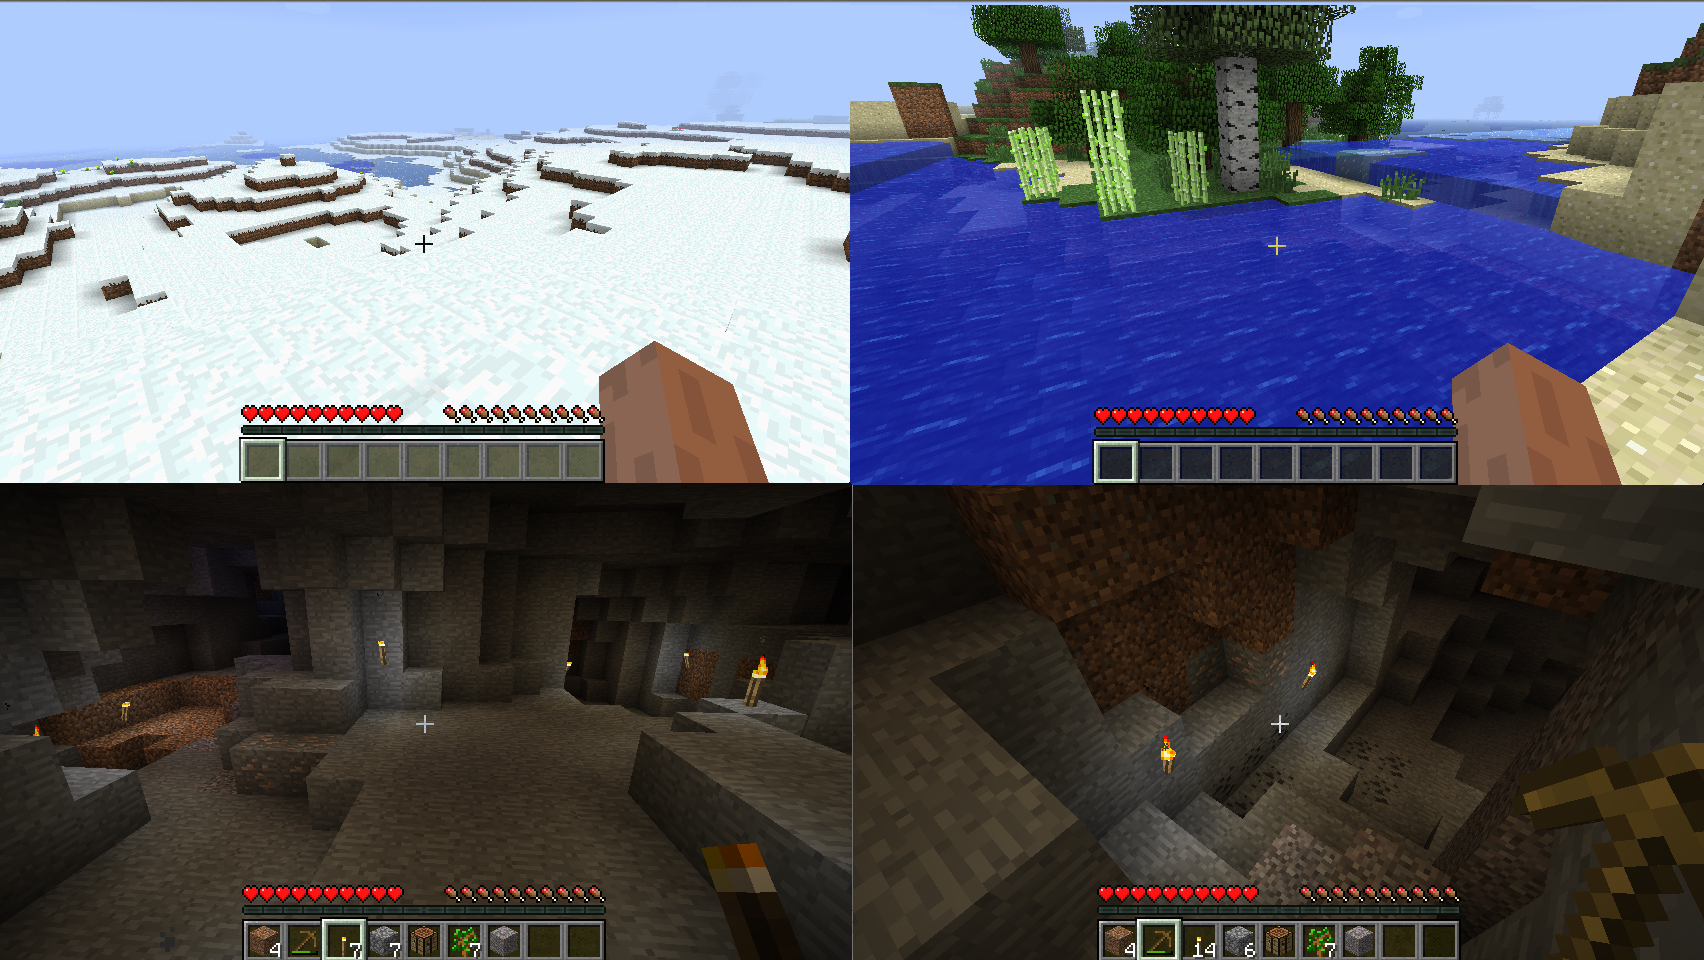
\includegraphics[width=0.92\textwidth]{images/minecraft.png}
\caption{Procedural level design in Minecraft.}
\end{figure}

A game similar to Minecraft that also uses PCG is Terraria. Like Minecraft, it also revolves around randomly positioned blocks, with the main difference being that it's a 2D game. Terraria is a lot more focused on generating content other than terrain. In Terraria players can encounter numerous different types of enemies. They can also find treasures in vases and chests that are randomly scattered across the world.
\begin{figure}[h!]
\centering
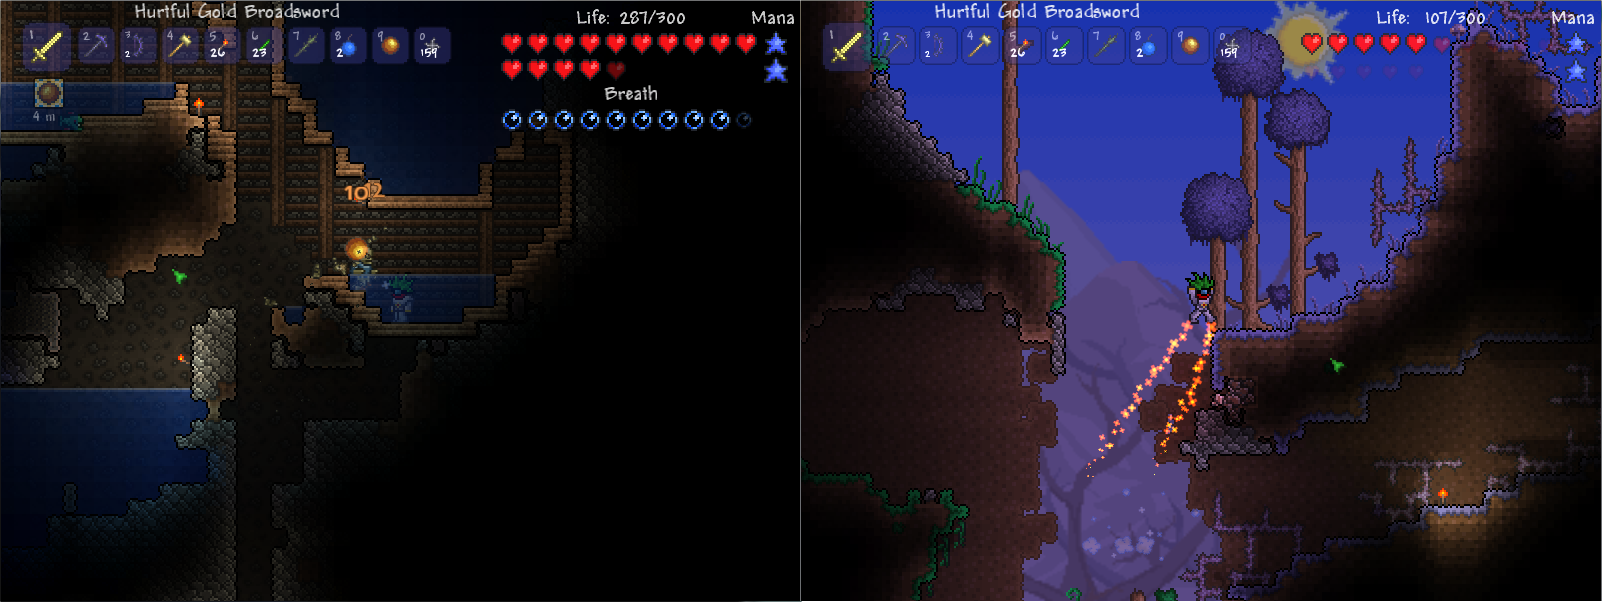
\includegraphics[width=0.6\textwidth]{images/terraria.png}
\caption{Terraria is a 2D game inspired by Minecraft which also utilises PCG.}
\end{figure}

	\section{Advantages}
The programmatic approach presents various advantages over level designing. The two major advantages are:
\begin{enumerate}
\item {\bf Time:} Naturally, level designing is a very time-consuming process. However, computers are much faster than humans. Once a good level generator is developed, it can potentially generate an infinite amount of levels in a very short time-span. 

\item {\bf Amount of content:} As a direct result from the time constraint, level generation offers far more content. Video games with a fixed level design offer far less re-playability than those with procedural level generation because the game will get boring and predictable after a while. Level generation can allow a completely different feel to the game every-time it's played and can offer seemingly endless content \citep{DBLP:conf/aiide/ComptonM06}.
\end{enumerate}

Notably, other minor advantages can emerge from this programming approach. For instance, the total memory consumption of the game when distributed could be less, because content is generated on the fly when needed and doesn't have to be packed in the distribution medium \citep{DBLP:journals/tciaig/TogeliusYSB11}.


	\section{Disadvantages}
Although PCG can makes things interesting in a video game there are major downsides to it:
\begin{enumerate}
\item {\bf Unrealic:} Because the levels are generated at random by a computer they are effectively only mimicking a real-life environment. Real-life scenarios are too complex to express and are therefore based on approximate models. If these models are not accurate enough then generated content will have obvious unrealistic features.

\item {\bf Specificity:} The behaviour of a content generation algorithm should be specific to the desired result. For example: generating a natural environment such as a forest will require an algorithm that is substantially different to an algorithm used to generate a city. Generalisation is not always possible and environments with mixed characteristics will have to incorporate multiple techniques, making them more complex.

\item {\bf Repetition:} PCG algorithm generally rely on pre-defined assets of sorts to increase the realism of an environment. For example: an algorithm used to generate a desert would probably utilise some artwork, such as one or more sand pictures to diffuse a texture. Even if the algorithm doesn't use any artwork then the formulas used to model the environment will generate sections that are noticeably similar.
\end{enumerate}

All of these issues can be reduced in some ways. To make the environment more realistic, we need to rely on a lot of artwork to make the result more convincing. However, if we rely too much on pre-determined assets then it will increase repetition and the generated content will lose its uniqueness. We cannot produce an infinite amount of pre-determined assets and must rely on mathematical functions with a wide range to effectively reduce repetition. As for specificity, the best way to counter this is to write base code that can be extended by different algorithms.


	\section{Statement of Problem and Aims}
We know now that PCG can potentially be advantageous to game developers. PCG suffers from three major issues and amongst those there is one that seems to be more neglected than others: Specificity. Maximising realism whilst reducing repetition tends to be the priority for game developers because those two issues directly affect the visual quality of game. 

In this thesis, the primary focus will be to keep the algorithm as general as possible. In order words, the problem of specificity will be tackled more directly than the others. The aim of the project is to conceive a framework that is entirely independent and capable of being re-used in any game that requires that kind of environment. The framework should be able to support the following key features:
\begin{itemize}
\item Using a solid mathematically to model generate dungeon-like environments. This model should be abstract and extendible.
\item Procedurally model the generated environment into a 3D mesh.
\item Render the environment and provide means for the user to interact with the environment.
\end{itemize}
\chapter{PCG Techniques}
The most important thing to keep in mind when working with PCG is that different environments require different PCG methods. Before we start looking specifically into dungeon generation we must first identify the major PCG techniques to decide which one fits best.

\section{Genetic algorithms}
Togelius et al. distinguishes two types of content generation. The first is with the use of a {\em constructive algorithm} that consists of generating the content in a single run with little or no backtracking \citep{springerlink:10.1007/togelius1}. The other method, referred to as {\em generate-and-test algorithms}, carries out a number of attempts and select only the candidates that satisfy a set of tests \citep{springerlink:10.1007/togelius1}. Typically, such algorithms are more complicated and more time-consuming, however if handled with care they can provide results in only a fraction of a second \citep{DBLP:conf/cig/TogeliusPBWHY10}. Due to the nature of genetic algorithms, they tend to provide very good results for generating outdoor terrain or, in other words, generating the height-map of a level \citep{DBLP:conf/gecco/RaffeZL11}.

Genetic algorithms are essentially generate-and-test algorithms \citep{springerlink:10.1007/togelius1}. A genetic algorithm can metaphorically be described as:
\begin{quote}
``Genetic Algorithms mimic real life evolution, in particular based on Darwin’s theory of Natural Selection" ... ``Features change over time due to natural mutations and mutual heritance." \citep{DBLP:conf/ACMace/MouratoSB11}.
\end{quote}

The idea of a genetic algorithm is to create a series of candidates, selectively pick out the best ones and then repeat this process until a satisfactory solution emerges \citep{DBLP:conf/ACMace/MouratoSB11}.

\begin{figure}[h!]
  \centering
    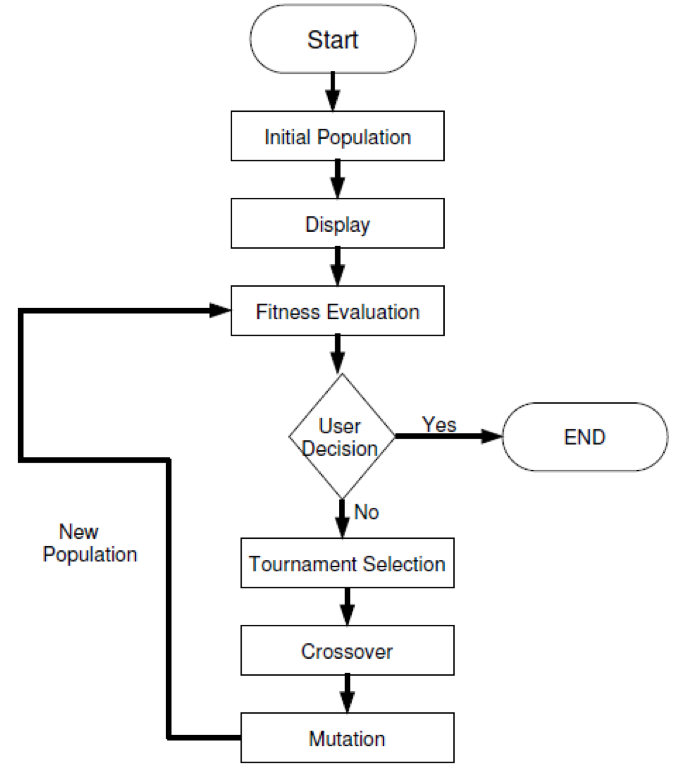
\includegraphics[width=0.4\textwidth]{images/genetic-flowchart.png}
\caption{Flowchart representation of a genetic algorithm. Image sourced from \citep{DBLP:conf/cec/WalshG10}}
\end{figure}

\subsection{Fitness function}
The key element in any genetic algorithm is the {\em fitness function}, which is the function that defines `how good' a solution is. This function is used to test the validity of a candidate \citep{DBLP:conf/evoW/SorensonP10}. 

Based on the usage of this fitness function, we can obtain entirely different results. Sorenson and Pasquier demonstrated that it is possible to conceive a generic framework for PCG by considering the fitness function as the amount of fun a level can convey. Naturally, the concept of fun is a rather abstract concept from a mathematical point of view. Their fitness function is dependant on a challenge measurement function, which is specific to a certain genre of game. This abstraction on the fitness function allows the algorithm to generate content both for a 2D side-scrolling platform game (such as {\em Super Mario Brothers}) as well for a dungeon-like top-down view game (such as {\em The Legend of Zelda}) \citep{DBLP:conf/evoW/SorensonP10}.

The fitness function can measure anything based on what is required. For instance, using a fitness function that measures fun is probably more viable for creating the environment of a video game \citep{DBLP:conf/evoW/SorensonP10}, whereas a function that measures the aesthetics of a terrain is more suited if the algorithm is intended to generate beautiful terrain \citep{DBLP:conf/cec/WalshG11}.

\subsection{Genetic operators}
When candidates are selected they will evolve in some way. Raffe et al. distinguish two kinds of selections: {\em parent selection} and {\em gene selection} \citep{DBLP:conf/gecco/RaffeZL11}. Distinguishing between the two is not necessary, but in doing so one gets an increased amount of control on how the algorithm behaves \citep{DBLP:conf/gecco/RaffeZL11}.

\paragraph{Mutation} This is where a single candidate evolves on its own, meaning certain genes will change into different values. The mutation can be random or selective \citep{DBLP:conf/ACMace/MouratoSB11}.
\paragraph{Cross-over} This is where two candidates are mixed together. How these two candidates are mixed depends on the type of problem being solved and the desired result \citep{DBLP:conf/ACMace/MouratoSB11}.

\section{Search-Based}
Search-based content generators are based around viewing the generation process as a search problem with a starting state, a goal state and several randomised intermediate states. They can be used to generate different kinds of content depending on how the algorithm is used. According to Togelius et al., Search-based procedural content generation (SBPCG) algorithms are generally based upon some sort of evolutionary algorithm \citep{DBLP:conf/cig/TogeliusPBWHY10}.

Togelius et al. define a search-based algorithm as such:
\begin{quote}
``Search-based procedural content generation (SBPCG) is a particular type of generate-and-test PCG, where the generated candidate content is not simply rejected or accepted by the test but graded on one or several numeric dimensions, and where a search algorithm is used to find better content based on the evaluations of previously generated content."\citep{DBLP:conf/cig/TogeliusPBWHY10}
\end{quote}

A SBPCG algorithm was used by Togelius et al. to procedurally generate maps for the Real-time strategy game StarCraft. These maps are generated by using in-game objectives such as mineral fields and geysers as the goals of the search-problem \citep{DBLP:conf/cig/TogeliusPBWHY10}.

However, search-based procedural generation techniques can also be used for generating random maze-like structures using a method suggested by Ashlock et al. This method used an algorithm that consists of visiting parts of the maze at random using a fitness function. An interesting feature about this method is that it's independent from the representation of the maze. The authors demonstrate the execution on three kinds of representations \citep{DBLP:journals/tciaig/AshlockLM11} :
\begin{itemize}
\item {\bf Direct:} Represented by a grid where each element is a bit that represents either a wall, by the value 1, or a walk-able area, by the value 0.
\item {\bf Indirect positive:} Values are stored in an array and represent the walls of the maze.
\item {\bf Indirect negative:} Values are stored in an array and represent the empty space (rooms and corridors) of the maze.
\end{itemize}
Naturally all these representation can be expanded to include more possible values and, in doing so, allow different kinds of terrain / walls across the maze \citep{DBLP:journals/cim/AshlockLM11}.

Ashlock et al. also clearly illustrate the importance of the fitness function. Here are some examples of different results obtain by merely using a different function \citep{DBLP:journals/tciaig/AshlockLM11}:
\begin{itemize}
\item {\bf Exit Path Length Fitness ($F_1$):} The function causes the maze to be composed of a single long path.
\item {\bf Primitive Re-convergence Sum Fitness ($F_2$):} This can produces a maze with dead-ends, also referred to as cul-de-sacs.
\item {\bf Isolated Primary Re-convergence Sum Fitness ($F_3$):} This function produces a maze with paths that split off and meet up again at the end.
\end{itemize}

\begin{figure}[h!]
  \centering
    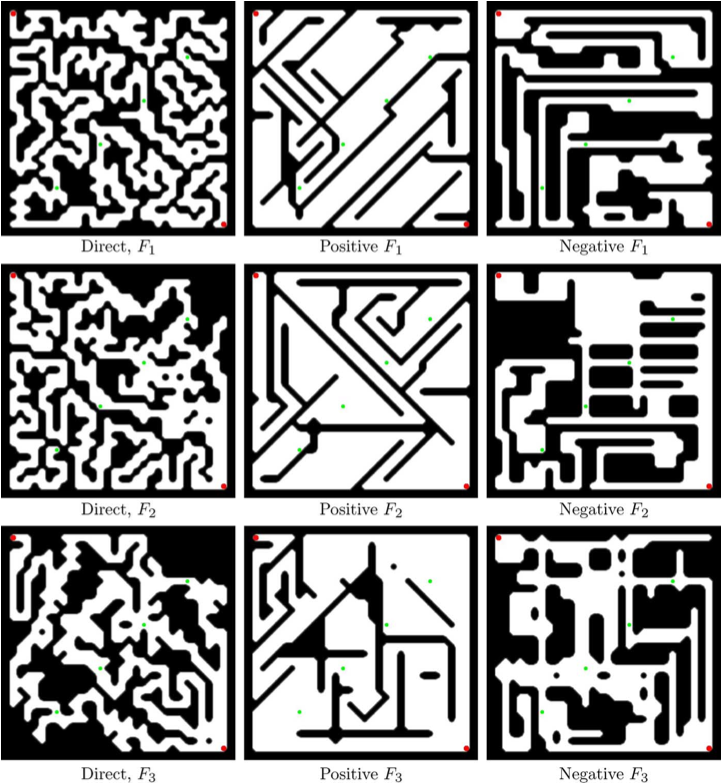
\includegraphics[width=0.50\textwidth]{images/ashlockMazes.png}
  \caption{An illustration of the various types of mazes generated \citep{DBLP:journals/tciaig/AshlockLM11}.}
\end{figure}


\section{Rhythm-Based} 
In platform-genre video games such as {\em Super Mario} and so forth, the aspect of timing and rhythm is particularly important \citep{DBLP:journals/tciaig/SmithWMTMC11}. Such games revolve around the fact that the player must hit the right keys at the right time. One example of timing is the act of running and jumping to get across a gap in the level. If the player jumps too early, they will not reach the next platform and fall. If the player presses the jump button too late then their character would fall before starting the jump \citep{Smith:2008:FAP:1401843.1401858}.

\begin{figure}[h!]
  \centering
    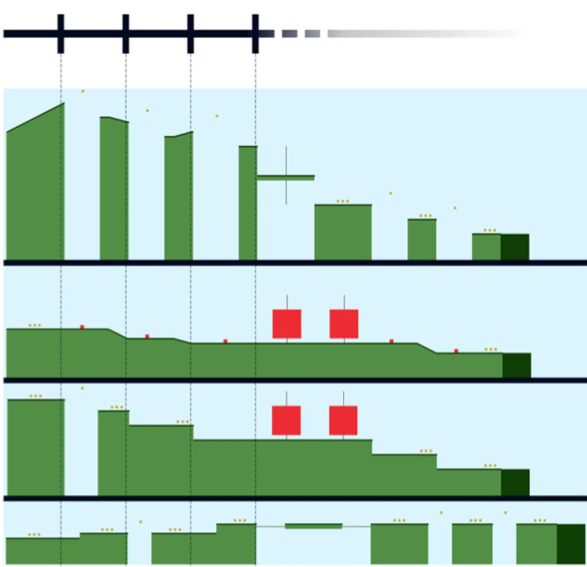
\includegraphics[width=0.28\textwidth]{images/rhythm.png}
  \caption{Platform game level generation using a rhythm-based technique \citep{DBLP:journals/tciaig/SmithWMTMC11}}
\end{figure}

A level generator called Launchpad has been designed based on this key concept of rhythm \citep{DBLP:journals/tciaig/SmithWMTMC11}.
The generator creates sections that are either `jump' or `walk'. The frequency of these jumps is defined by the rhythm of the algorithm. Additionally the length and height of the terrain will vary at random \citep{DBLP:journals/tciaig/SmithWMTMC11}. 

N. Shaker et al. then conceived an optimisation to such an algorithm using Artificial Intelligence (AI) \citep{DBLP:conf/aiide/ShakerYT10}. The algorithm consists of first generating a level at random. Afterwards, an AI player plays through the level and the action's of that player are recorded. Based on these actions the algorithm will then optimise the level to make it more enjoyable.

Needless to say, such algorithms are directed specifically to platform games and are not directly applicable to other genres. Although these algorithms are aimed at 2D games a 3D implementation could still be possible but would involve a large increase of constraints.


\section{Occupancy-regulated}
The main disadvantage with purely randomised levels is that things can look a little bit unnatural or lack the sense of creativity. Human-designed levels present the advantage of being more unique and more suited to the type of game developed \citep{DBLP:conf/cig/MawhorterM10}. Mawhorter and Mateas have suggested an occupancy-regulated algorithm that allows random levels to be used whilst maintaining liberty and control for human level designer.

The authors summarise the algorithm as such:
\begin{quote}
``Occupancy-regulated extension works by assembling a level using chunks from a library." \citep{DBLP:conf/cig/MawhorterM10}.
\end{quote}

\begin{figure}[h!]
  \centering
    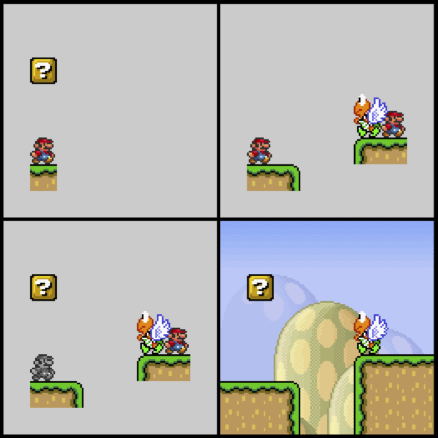
\includegraphics[width=0.35\textwidth]{images/mario.png}
  \caption{An illustration of Mawhorter and Mateas' algorithm. The two top panels are individual chunks. The lower left panel presents the two chunks mixed. The lower right panel is the result after post-processing. Image source: \citep{DBLP:conf/cig/MawhorterM10}}
\end{figure}


The idea is that level designers need only to design small key sections of the level that are referred to as `chunks'. Each chunk consists primarily of empty space along with certain aspects of the game, such as a jump, an NPC spawn point and so forth. Along with this, each chunk has a set of pre-defined locations where the players can legally situate themselves. These locations are called anchors \citep{DBLP:conf/cig/MawhorterM10}.

The algorithm then uses these anchors to blend several chunks together. It will take one anchor from each chunk and maps those anchors to the same location in the world. Once the level is complete the post-processor will fill the empty areas with additional components such as decorations and un-passable terrain. \citep{DBLP:conf/cig/MawhorterM10}.

This method can produce some very interesting and enjoyable levels but can cause a lot of repetition if the chunk-library is too small \citep{DBLP:conf/cig/MawhorterM10}. For example, players of the game title Diablo 3 will notice a lot of identical rooms being repeated. This suggests that this title uses some kind of occupancy-regulated algorithm, although there is no real evidence to support this.


\section{Procedural Modelling}
Procedural modelling is special kind of PCG in which the algorithm generates a 3D mesh. Algorithms that we have explored until now focused on designing the structure of a maze, or the layout of platforms. However, none of these were particularly focused on the modelling aspect of an environment.

In an article published in 2003 the authors present an interesting way of procedurally modelling skyscrapers in real-time \citep{DBLP:conf/graphite/GreuterPSL03}. The method consists of building the floor-plan by piling primitive shapes on one another and obtaining the union of that region \citep{DBLP:conf/graphite/GreuterPSL03}. The border of this floor-plan is then extruded to form a 3D object and this process is repeated for the succeeding stories \citep{DBLP:conf/graphite/GreuterPSL03}. This method is a simple, elegant and a cost-efficient way of procedurally modelling a random room. A method like this could be used to generate the rooms of a dungeon.

Procedural modelling can used also be done using L-systems. Parish and M\"uller suggested a method of using extended L-systems to generate the road map in the form of a graph. They then use L-systems again to procedurally construct the geometry of the buildings. The authors also propose a method of procedurally generating the textures of the meshes, which effectively causes a wider range of building styles to be generated \citep{Parish:2001:PMC:383259.383292}.

\begin{figure}[h!]
  \centering
    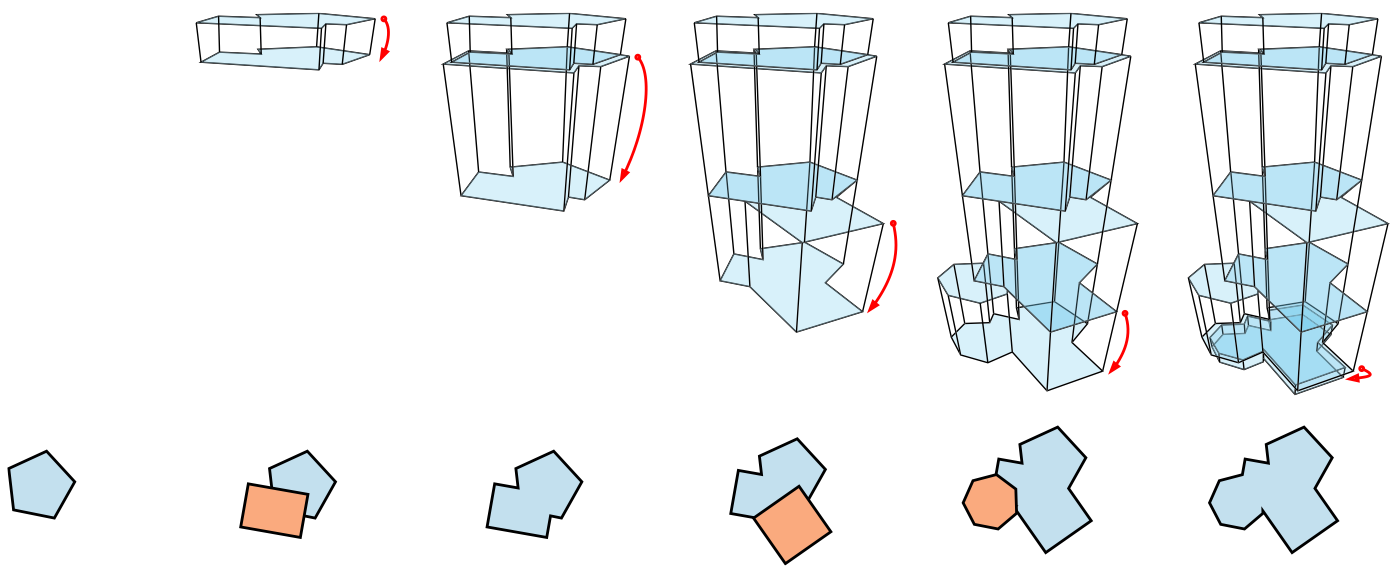
\includegraphics[width=0.75\textwidth]{images/floorplan.png}
  \caption{The various steps of the floor-plan generation. Image source: \citep{DBLP:conf/graphite/GreuterPSL03}}
\end{figure}

Another interesting topic is how to interconnect structures together through bridges, staircases and so forth. One simple approach to link two structures together is by simply interconnecting them linearly using a shape such as a box for instance \citep{DBLP:journals/cgf/KrecklauK11}. However this may not always look convincing and is not sufficient to generate interconnections with curves and deformed pieces \citep{DBLP:journals/cgf/KrecklauK11}. 

Various methods exist to generate non-linear interconnections. One example is to use a rigid chain, a structure which is best described as a:
\begin{quote}
``sequence of revolute (rotational) and prismatic (translational) joints." \citep{DBLP:journals/cgf/KrecklauK11}
\end{quote}
The angles and positions of these joints can be calculated through the use of Inverse Kinematics (IK) \citep{DBLP:journals/cgf/KrecklauK11}. However when solving an IK problem a solution may not always exist, such as if the target point is out of arm's reach \citep{Tolani2000353}. A good IK solving algorithm must not only be able to find a solution if one exists, but it should also detect and report if a result is unreliable or no solution could be found \citep{Tolani2000353}.

Hahn et al. have developed a method to generate the interior content of a building with multiple floors in real-time. It uses lazy execution to insure that content is only generated once the player approaches a portal near an un-explored region. They use a number of strict generation rules to follow when generating content in order to do so efficiently. The algorithm uses a {\em generation tree} to divide the large space into floor divisions, hallway divisions, and room cluster division \citep{Hahn:2006:PRB:1183316.1183342}.
\chapter{Random Number Generation}
It is obvious that the aspect of randomness is a crucial factor in procedural content generation. Random numbers are required for countless reasons. They can be used to pick a random element in a set or to assign a random value to a variable. Generating random numbers is a concept that has been in the field of research for many years and, although solutions exist, it remains a delicate task. 

In most cases a pseudo-random number generator (PRNG) can be used to generate numbers, although these do not provide a true random result. The term ``pseudo-random" is used to define a sequence of deterministic generated numbers with a distribution that closely resembles that of random variable. Because of the fact that random numbers generated by a PRNG are defined by a mathematical formula, poor PRNG algorithms suffer from several issues such as predictability and dependent distributions \citep{frieze_lcg}.

\section{Linear Congruential Generators}
Linear congruential generators (LCG), proposed several decades ago by D. H. Lehmer, are amongst the oldest and most common PRNG \citep{park_miller}. Requiring nothing but a single variable and a simple formula for generating numbers, they are considered very memory and time-efficient. Their space and time complexity are of order $\bigo{1}$ \citep{Knuth_art2}.

As direct result of their simplicity and efficiency, LCGs are often used in certain applications such as simulations where a satisfactory result that ``looks good" is required. However they present the disadvantage of producing predictable and dependent variables \citep{frieze_lcg}.

\subsection{Recurrence relation}
Linear congruential generators are mathematically described by the following recurrence relation:

\[ X_{n+1} = (a X_{n} + c) \modulo M \]

This recursive formula is used to generate a sequence of numbers $\{X_0, X_1, X_2,...\}$ with a seemingly random uniform distribution \citep{Knuth_art2} where each variable represents the following (as explained by \citep{hamid_lcgSecurity}):
\begin{itemize}
\item $X_{n+1}$ is the next ``random" number in the sequence $\{X_0, X_1, X_2,...\}$. It is referred to as \texttt{next()} in some implementations such as .NET's \texttt{System.Random} class \citep{System.Random} or Java's \texttt{java.util.Random} class \citep{java.util.Random}.
\item $M$ is called the {\em modulus}, generally a large prime number \citep{park_miller}
\item $a$ is called the {\em multiplier}. $0<a<M$
\item $c$ is called the {\em increment}. $0 \leq c<M$
\item The operation $ \modulo $ is called the modulo and defines the remainder of an integer-division.
\end{itemize}

\subsubsection{Seed}
As with all recurrence relations, the formula requires a starting point. In other words the formula should be defined as the following:

\begin{align}
 X_{0} &= k \nonumber \\
 X_{n+1} &= (a X_{n} + c) \modulo M \nonumber
\end{align} 

Where $k$ is a constant. The initial value $X_0$ is called the {\em seed} of the generator \citep{hamid_lcgSecurity}. In some implementations such as the  \texttt{java.util.Random} class the variable $X_n$ is also called the seed \citep{java.util.Random}, although generally speaking the term {\em seed} refers to $X_0$. 

It is trivial yet important to note that LCGs are ironically deterministic. Two identical LCGs (meaning the values for $a$, $c$ and $M$ are the same) will give exactly the same sequence of numbers if the seed is the same for both LCGs. This is a key concept in PRNG algorithms. Any program that utilises a pseudo-random number generator will provide exactly the same result if all given inputs (including the seed) are the same \citep{Knuth_art2}.

This is an obvious problem since the aim of any PRNG is to mimic the aspect of non-determinism. In order to obtain a different result we require a different seed. Typically, whenever a random seed is needed the computer's time can be used as the seed because this is guaranteed to be unique. The clock time is a feature related to time, which breaks the determinism of the LCG and provides a more unpredictable result \citep{Knuth_art2}.

\subsubsection{Period}
Another problem with LCGs is that the sequence produced is essentially always the same even when using a different seed. This issue is easiest to explain with the use of an example. 

\begin{itemize}
\item Let us consider two generators $L_X$ and $L_Y$ that differ only by their seeds.
\item Let $X_0$ and $Y_0$ be the seeds of $L_X$ and $L_Y$ respectively.
\item Let $a = 3,\;c = 1,\;M = 7$. These values for $a$, $c$ and $M$ are most certainly non-ideal but are used only for the purpose of demonstration.
\end{itemize}

We can calculate the numbers generated by the first LCG $L_X$ when its seed is $X_0 = 1$ for instance:

$$ \{X_0, X_1, X_2, ...\} = \{1,\,4,\,6,\,5,\,2,\,0,\,1,\,4,\,6,\,5,\,2,\,0,\,1,\,4,\,...\} $$ 

We can do the same for the second LCG $L_Y$ with a different seed $Y_0 = 5$:

$$ \{Y_0, Y_1, Y_2, ...\} = \{5,\,2,\,0,\,1,\,4,\,6,\,5,\,2,\,0,\,1,\,4,\,6,\,5,\,2,\,...\} $$ 

Here we notice two things:
\begin{itemize}
\item The infinite sequence produced by $L_Y$ is nothing more than the sequence from $L_X$ with an offset. In mathematically terms: 
\\ $ \{X_0, X_1, X_2, ...\} = \{Y_3, Y_4, Y_5, ...\} $
\item The infinite sequence produced by both $L_X$ and $L_Y$ is simply an infinite repetition of a finite sequence
\end{itemize}
Both of these observations are due to the mathematical determinism of the method. In other words, given a certain input to the LCG, say $X=1$, the result will always be 4.

\subsection{Advantages and Disadvantages}
\paragraph{Advantage} LCGs are famous for their efficiency and simplicity. They are easy to understand and implement. Requiring nothing more than a few simple operations such as bit-shifts and additions, they are computationally cheap \citep{wang_review} and only require a single 16-bit word of storage at-least \citep{yu_random}. Pierre L'Ecuyer has shown that larger word sizes can be used to provide more decent results \citep{lecuyer_tables}. Regardless of word-size used a single word is negligible on modern machines.

\paragraph{Disadvantages} 
As demonstrated by Pierre L'Ecuyer, LCGs can give satisfying results in certain applications such as simulations \citep{lecuyer_lcg_k1}. However, the quality of the pseudo-random numbers is very sensitive to the values assigned to its parameters $a$, $c$ and $M$. Bad choices for these parameters have historically lead to LCGs with inadequate results \citep{li_ooRandom}. Finding good coefficients for a LCG is very difficult and has been in the field of research for many years \citep{park_miller}. Generally in most applications, a known and reputable LCG will be used instead of innovating a new one. For instance, the LCG used in Java's \texttt{java.util.Random} class is based on the algorithm discussed by Donald E. Knuth in the {\em The Art of Programming: Volume 2} \citep{Knuth_art2}.

Aside from the concern for the quality of the result, LCGs also has a major concern regarding security. LCGs are notorious for their predictability even if the coefficients provide decent results \citep{hamid_lcgSecurity}. Plumstead has shown that the multiplier $a$ and multiplier $M$ can be inferred when a certain number of pseudo-random bits are revealed \citep{plumstead_predicting}. Therefore, using merely a fragment of a LCG's output, it is possible to predict the sequence of pseudo-random bits without knowing the coefficients $a$ and $M$ \citep{frieze_lcg}. Even worse, once the modulus becomes known we can predict the output with almost perfect certainty as demonstrated by Jacques Stern \citep{Stern_lcgInsecure}. Needless to say, this is a big concern for security because a high degree of unpredictability is required. Therefore LCGs are un-recommended for the use of cryptography. Some suitable alternatives derived from LCGs can be used for cryptography. An example is the Blum Blum Shub algorithm \citep{BlumBlumShub-1}.

\subsection{Constraints for good LCGs}
The aim of a number generator is to provide a sequence of numbers with good statistical properties and randomness \citep{hamid_lcgSecurity}. Naturally good randomness is required for simulation, but it has been shown by \citep{Knuth_decipher} and \citep{plumstead_predicting} that a LCG is more difficult to decipher if its output possesses good statistical randomness. This  makes statistical randomness the key element when designing a number generator.

Another essential feature for LCGs is the concept of full-period. A full period means that all values $0\leq X<M$ are generated once before the LCG returns to its initial state (i.e. it re-generates the initial seed) \citep{Knuth_art2}. Our previous example with the coefficients $a = 3$, $c = 1$, $M = 7$, $X_0=1$ is not a full-period LCG because the period generated does not include $3$:
\[\{1,\,4,\,6,\,5,\,2,\,0,\,1,...\}\]
A full-period LCG with a modulus $M=7$ would generate a period that includes all the numbers $\{0,\,1,\,...,\,6\}$. Donald Knuth has stated that a LCG has a full-period if and only if \citep{Knuth_art2}:
\begin{itemize}
\item The coefficients $c$ and $M$ are {\em relatively prime}, meaning they have no common dividers other than 1.
\item $a-1$ is divisible by all the prime factors of $M$.
\item If $M$ is a multiple of 4 then $a-1$ is so too.
\end{itemize}
However, full-period LCGs are not guaranteed to provide good results. In an example shown by Park and Miller they demonstrated this by using two similar number generators, both provided full-period sequences. These generators were given by formulas \((6 X \modulo 13)\) and \((7 X \modulo 13)\). However the former provided better statistical randomness, making it superior to the latter \citep{park_miller}.


\subsection{Examples of good and bad LCG}
Park and Miller suggested a good example of a LCG that provides adequate results. They refer to this LCG as the {\em minimal standard generator} \citep{park_miller}. This LCG uses the coefficients $M = 2^{31}-1$, $a = 7^5$ and $c = 0$. They claim that this LCG possesses both the full-period and statistical randomness properties. Additionally they also state that this LCG is easy to implement on nearly every computer system \citep{park_miller}.

\begin{quotation}
``We present the rationale for our choice of a minimal standard generator. We believe that this is the generator that should always be used -- unless one has access to a random number generator known to be better." \citep{park_miller}
\end{quotation}

Unfortunately good LCGs are difficult to find and hence there are many LCGs that suffer from certain defects \citep{park_miller}. Notably any number generator with a modulus of the form $M=2^n$ will suffer from an effect where lower bit are less significant and causes problems. For instance, the full-period mixed generator on UNIX platforms called \texttt{rand()} suffers from an issue where  the distribution of the lower bits is non-random \citep{park_miller}. The generator \texttt{rand()} used the parameters $a=1103515245$, c=$12345$ and $M=2^{31}$ \citep{park_miller}.

Another poor example of a LCG which suffers from the same effect that causes a defect in \texttt{rand()} is the random number generator in Turbo Pascal. The parameters used are $a=129$, $c=907633385$ and $M=2^{32}$, which is claimed to be even worse than the function \texttt{rand()} because the multiplier is simply too small \citep{park_miller}.

The worst example of any LCG must probably be the random generator known as RANDU. The coefficients are given by $a=2^{16}+ 3$, $c=0$ and $M=2^{31}$. These coefficients were chosen because they made the implementation of the algorithm very simple and it quickly became widespread \citep{park_miller}. However RANDU does not have a full period and the numbers generated have a distribution which is clearly non-random \citep{park_miller}.

\begin{quotation}
``...its very name RANDU is enough to bring dismay into the eyes and stomachs of many computer scientists!" \citep{Knuth_art2}
\end{quotation}

\section{Alternatives}
\subsection{Coupled Linear Congruential Generators}
In the attempt to make a PRNG that is efficient and cryptographically secure, Katti et al. suggested the use of Coupled Linear Congruential Generator (CLCG). This consists of using two LCGs with slightly different arguments to generate a sequence of bits. They show that breaking a CLCG is of complexity $\bigo{2^{2n}}$ where $n$ is the number of bits in the modulus $M$, which they consider as ``moderate security". However the authors confess that not all CLCGs pass the statistical tests of randomness, but they propose a modified version of CLCGs called dual-coupled LCG designed to provide statistically satisfying results. \citep{katti_coupledCG2}

\subsection{Mersenne twister}
Although LCGs generally provide adequate results they present major flaws in certain applications. One typical example is the Monte Carlo simulation that consists of repeatedly sampling data and testing them. Good statistical randomness is required in order for this simulation to work properly, LCGs simply don't have a level of randomness that is sufficient for a Monte Carlo simulation \citep{Itan-MonteCarlo}. In 1997, Makoto Matsumoto and Takuji Nishimura conceived a pseudo-random number generator known as the Mersenne twister. This method is optimised to provide statistical randomness and passes most statical tests \citep{DBLP:journals/tomacs/MatsumotoN98}. However this number generator on its own remains cryptographically insecure and shouldn't be used for this purpose, although it is possible to modify the algorithm to make it safe \citep{DBLP:journals/iacr/MatsumotoNHS05}.


\subsection{Blum Blum Shub}
PRNG algorithms such as LCG and Mersenne twister are fast and provide decent results. However, they are not cryptographically secure and are predictable. When considering randomness for security proposes, one must consider a different algorithm such as the {\em Blum Blum Shub} algorithm.

The name of the Blum Blum Shub algorithm is derived from its three creators Lenore Blum, Manuel Blum, and Michael Shub. \citep{BlumBlumShub-1} The formula used to generate pseudo-random bits is given as:

\[x_{n+1} = x^2_n \modulo M \]

Where $M$ is the product of two large prime numbers $p$ and $q$. The seed \(x_0 \notin \{0,1\} \) should be co-prime to $M = pq$ \citep{BlumBlumShub-2}.

This number generator is particularly useful in the field of cryptography because of its unpredictability. Predicting the output of the algorithm is possible, but it is a problem that is {\em computationally difficult} to solve. The problem is at-least as difficult as factorising $M$, which is an {\em NP-complete} problem \citep{BlumBlumShub-1}.

\pagebreak
\chapter{Maze and Dungeon Generation}
Maze and dungeon generation has been around for some time but sadly still lacks significantly in the field of research. Basic maze generation algorithms already exist but only few attempts have been made to push these generic algorithms to the next level. Most maze generation algorithms are specialised graph-traversal algorithms that use pseudo-random number generators to visit cells of the dungeon in a random order. This chapter will discuss precisely how these various algorithms work, what features can be added to enhance them and how to apply these algorithms in a 3D application such as a video game. The aim of this chapter is to conceive a framework for procedural dungeon generation with maximum re-usability. Despite being targeted at dungeon-like environments, the features discussed in this section remains generic and can be used as a starting point for any 3D application that needs to make use of it.

\section{Maze Generation}
\subsection{Understanding Search-problems}
It has been observed that there are a large number of PCG techniques that are useful for a number of different kinds of environments. To generate a dungeon-like environment such as in the {\em Dungeons \& Dragons} pen-and-paper game a decision needs to made regarding what technique should be used to base the framework on. Judging by the results of mazes produced by Ashlock et al. it appears as though the search-based generation technique could be very viable \citep{DBLP:journals/tciaig/AshlockLM11}. In this the kind result that's desired and therefore the algorithms that will be discussed throughout this chapter will essentially be search-based.

Before going any further it is vital to understand exactly what is meant by a {\em search-based} algorithm. The idea behind a search-based algorithm is to start at a given state called the {\em start} state. From that initial state we can {\em transition} into a set of new  states and from those new state transition into even more states and so forth. The aim of these search-based algorithm is to try find a state that matches the {\em goal} \citep{DBLP:conf/cig/TogeliusPBWHY10}. Note that when that the structure of search problems can be viewed as traversing a graph: the states of the problem are the {\em nodes} in the graph and the transitions from one state to another are the {\em edges}.

\subsection{Properties of a maze}
Fortunately, mazes already have a rigorous and well-established mathematically model and theory that can be used to our advantage. We can define many properties for a maze but the most important ones in procedural dungeon generation are the following:
\paragraph{Unicursal} A unicursal maze is one with no junctions. Solutions of a unicursal maze are long winded paths \citep{ThinkLabyrinth}. 
\paragraph{Perfect} A maze can be considered as perfect if it has no cycles and no inaccessible areas \citep{ThinkLabyrinth}.
\paragraph{River} The term river is used to determine how much a maze ``flows". If the river factor is low then the maze will tend to have many short dead ends, otherwise if the river factor is high the maze will have fewer but longer dead-ends \citep{ThinkLabyrinth}.
\paragraph{Bias} Biased mazes will have passages that tend to favour a specific direction \citep{ThinkLabyrinth}. 

All the mazes that are generated by the framework are initially {\em perfect}, although that can be changed if required. Some algorithms will produce {\em biased} mazed, although most of them tend to produce un-biased mazes. The faster algorithms tend to be the ones that produced biased mazes \citep{ThinkLabyrinth}.

\subsection{Maze generation as a search-problem}
\subsubsection{The Graph}
As explained previously, a search-problem traverses various nodes and can visit adjacent nodes by using incident edges of the graph. The graph in this case can be viewed as a grid with cells.

\paragraph{Cells (nodes)} The cells in the grid represent a position $(x,\,z)$ in the maze. These cells correspond to the nodes of the graph. If a cell in the maze has at least one adjacent wall missing then it can be referred to as a {\em floor} cell, otherwise if the cell is completely walled off then it can be referred to as a {\em wall} itself or a {\em block}.

\paragraph{Walls (edges)} Each cell has a place on the top, bottom, left and right to position a wall. Each wall is shared between cells, and hence these walls correspond to the edges of the graph. The walls can either be {\em on} or {\em off} (no wall), although in practice this domain can be expanded to include objects such as doors for instance. Note that the walls on the very edge of the grid are only mapped to a single cell which doesn't make sense from a theoretical point of view. So in theory we can assume that the walls on the border are linked to cells are permanently inaccessible and invisible, although in practice those invisible cells can be ignored.

\begin{figure}[h!]
\centering
 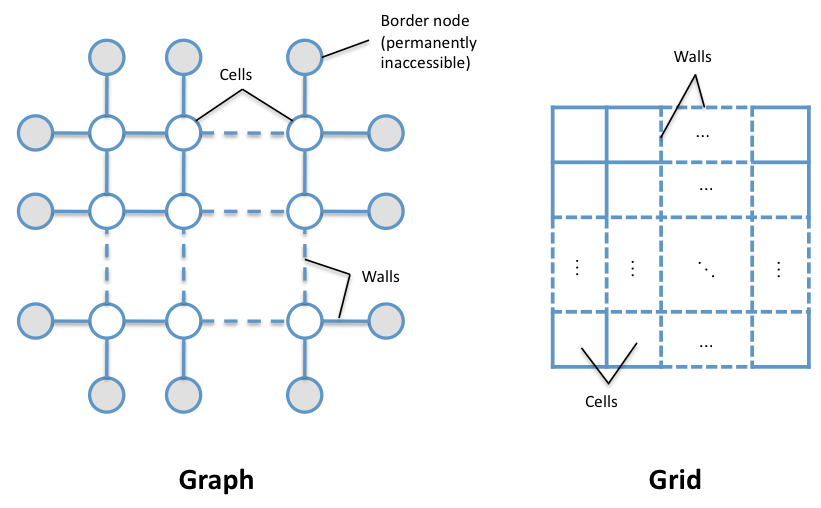
\includegraphics[width=0.87\textwidth]{images/graph-grid.png}
\caption{Graph and grid representations of the maze.}
\end{figure}

\subsubsection{The Goal}
In search problems the goal is a specific node that satisfies the desired conditions. Intuitively, one would believe that the start and end states of the search problem are the entrance (where the player starts) and the exit (where the player must get to) of the maze respectively. However, maze generators completely disregard the existence of such a concept. Instead, as explained by Pullen, all the maze generators will aim at generating perfect mazes and succeed to do so \citep{ThinkLabyrinth}. The two properties of a perfect maze, no cycles and no inaccessible cell, match exactly the definition of a {\em spanning tree\footnote{http://en.wikipedia.org/wiki/Spanning\_tree (Accessed on 15\textsuperscript{th} of July 2012)}} \citep{DBLP:journals/siamdm/Aldous90}. Therefore the goal of the search problem is to find a spanning tree.

\subsection{Depth-first search algorithm}
The depth-first search (DFS) algorithm is a simple way to implement maze generation. The classical depth-first search algorithm is modified slightly in this case to include the notion of random. Normally the children of a specific node are visited in an arbitrary order. However, in maze generation we will decide in which order the children should be visited at random. When visiting a new node the wall between the last visited cell and the new cell is removed. Upon reaching a node that has no un-visited children, we will backtrack and return to the last visited cell that still has unvisited children. The procedure is finished once there are no nodes to backtrack to (i.e. all the nodes have been visited).

Note that the DFS algorithm can be used for search-based algorithms. In this case however this is not the purpose of the DFS. We are simply using the DFS algorithm to create a random spanning tree. In other words, the DFS algorithm is only used to determine the transition from one state to another.

\lstAlgo
\begin{lstlisting}
Let M = the maze.
Mark each cell in M as "unvisited".
Let C = starting cell.
call DFS(C);

proc DFS(MazeCell C)
	while C has unvisited children do
		Pick random unvisited children D.
		Break walls between C and D.
		Mark D as "visited".
		call DFS(D);
	endwhile
endproc
\end{lstlisting}

We can observe that the depth-first search algorithm tends to provide mazes with a lot of very long paths (i.e. High river factor) \citep{ThinkLabyrinth}. This is because at the start of the algorithm very few cells are visited, hence the algorithm finds an unvisited child for each node more often than not, and hence backtracks very little. Therefore longer paths are generally caused because junctions are only created whilst backtracking which rarely occurs at the start. Later on, as the algorithm progresses, it finds more and more nodes with no unvisited children. So towards the end the algorithm tends to create more shorter paths and dead-ends become frequent.

\subsection{Prim's algorithm}
Another algorithm that is generally not used in search-problems is Prim's algorithm. Prim's algorithm is designed to find the {\em minimum spanning tree} of a {\em weighed undirected graph} using a {\em greedy method} \citep{Prim}. The idea behind the algorithm is to add the smallest weighed edge possible every iteration until all edges are included \citep{Prim}. The original algorithm is described below:

\lstAlgo
\begin{lstlisting}
proc Prim(Graph G)
	Mark each vertex in G as "unvisited".
	Let Es = All the edges of G.

	while (Total number of unvisited vertices) != 0 do
		Remove smallest weighed edged E from Es.
		Let C1, C2 = Vertices adjacent to E.
		
		if (E has at least 1 unvisited node) then
			Mark C1 and C2 as "visited".
			Add E to Es
		endif
	endwhile
	
	return Es // minimum spanning tree
endproc
\end{lstlisting}

Although Prim's original algorithm operates on the edges of the graph, it is possible to operate on adjacent nodes too \citep{DSAJ-4}. The modified version of Prim's algorithm for maze generation is expressed below:

\lstAlgo
\begin{lstlisting}
proc Prim(Maze M, MazeCell Start)
	Mark each cell in M as "unvisited".
	Let the set Cs = {Start}
	Mark Start as "visited".

	while Cs is not empty do
		Let C = random element of Cs.
		if (C has un-visited children) then	
			Let D = random un-visited child of C.
			Mark D as "visited".
			Break wall between C and D.
			Add D to Cs.
		else
			Remove C from Cs
		endif
	endwhile
endproc
\end{lstlisting}

Note that this modified version does not have the notion of {\em weight}. In the original algorithm we simply pick the edge with the smallest weight. However, in maze generation, we need to pick out a random edge from the set of available edges. From a conceptual point of view, the weights are assigned ``on the fly" and a random edge picked out as the minimum. 

Because of the nature of Prim's algorithm, the mazes constructed will look more ``spread out" than the depth-first search. In other words Prim's algorithm has the tendency to avoid creating very long paths \citep{ThinkLabyrinth}.

\subsection{Kruskal's algorithm}
Like the Prim's algorithm, Kruskal's algorithm is another greedy algorithm used to find the minimum spanning tree of a weighed undirected graph \citep{Kruskal}. The algorithm works by finding two unconnected trees in a {\em forest} and connecting them by removing the smallest weighed edge. The term {\em forest} refers to a set of trees that are not interconnected \citep{DSAJ-4}. The modified maze-generation version of the algorithm is given by:

\lstAlgo
\begin{lstlisting}
proc Kruskal(Maze M)
	Let F = Empty forest (set of trees).
	
	for each cell C in M
		Add the tree {C} to F.
	endfor
	
	for each wall W in M (in randomised order)
		Let C1, C2 be the two nodes connected by W.
	
		Let T1 = the tree in F that includes C1.
		Let T2 = the tree in F that includes C2.
		
		if T1 != T2 then
			Remove T1, T2 from F.
			Let G = T1 + T2 + W  // Connect T1 and T2.
			Add G to F.
		endif
	endfor
endproc
\end{lstlisting}

Because Kruskal's algorithm and Prim's algorithm both compute the minimum spanning tree they tend to provide mazes that look very similar to one another \citep{DSAJ-4}.

\subsection{Other algorithms}
Essentially, any algorithm that calculates a spanning tree of a graph can be used to generate a maze and several different algorithms exist \citep{AAJarai}. Other algorithms not based on spanning trees can also be used \citep{ThinkLabyrinth}. Pullen has enumerated the various different known algorithms that can be used in maze generation. However these other algorithms expose the inconvenience of being either slow or {\em biased} (meaning the maze has the tendency to follow a certain direction) \citep{ThinkLabyrinth}. 

\subsubsection{Aldous-Broder algorithm}
The Aldous-Broder algorithm got its name from its two creators: David Aldous and Andrei Broder \citep{DBLP:journals/siamdm/Aldous90}. The idea behind the algorithm is to generate a random {\em uniform spanning tree} as opposed to the minimum spanning tree from Prim and Kruskal's algorithms \citep{DBLP:conf/focs/Broder89}. A uniform spanning tree is defined as a spanning tree such that each edge has a uniform probability of getting picked\footnote{http://en.wikipedia.org/wiki/Uniform\_spanning\_tree (Accessed 16\textsuperscript{th} July 2012)}. The algorithm is expressed below:

\lstAlgo
\begin{lstlisting}
proc AldousBroder(Maze M, MazeCell Start)
	Initialize M such that all cells are "unvisited".
	Let C = Start.
	
	while M has unvisited cells do
		Let D = random neighbor of C.
		
		if D is unvisited then
			Mark D as "visited".
			Break wall between C and D.
			Let C = D.
		else if there is no wall between C and D then
			Let C = D.
		endif
	endfor
endproc
\end{lstlisting}

Because of the random nature of Aldous-Broder algorithm, it tends to produce mazes that are less biased and with a lower river factor than any other maze. However the algorithm is, on average, much slower than any other maze generation algorithms and isn't even guaranteed to terminate \citep{ThinkLabyrinth}.

\subsubsection{Wilson's algorithm}
This algorithm is an improved version of the Aldous-Broder algorithm and produces mazes that are the same \citep{ThinkLabyrinth}. However, Wilson's algorithm is much faster because it uses certain optimisation when retracing \citep{DBLP:conf/stoc/Wilson96}. On average, Wilson's algorithm is about 5 times faster than Aldous-Broder's algorithm, but 2 times slower than other algorithms \citep{ThinkLabyrinth}. 

\subsubsection{Hunt and Kill algorithm}
The Hunt and Kill algorithm is similar to the depth-first search algorithm; it differs only in the sense that it doesn't have backtracking. Instead, the algorithm starts in {\em Kill} mode and visits random cells breaking walls as it goes along just like the depth-first algorithm. However, once it reaches a dead-end it enters {\em Hunt} mode and scans the whole maze from top to bottom trying find an unvisited cell situated near a visited one; this substitutes the backtracking. It then breaks the wall between these two cells and returns to Kill mode. The algorithm is finished once the Hunt mode fails to find an unvisited cell \citep{ThinkLabyrinth}.

\subsubsection{Growing Tree algorithm}
The Growing Tree algorithm is very simple. It involves adding newly visited cells into a list and removing them once they have no more neighbouring unvisited cells. The algorithm simply picks a cell from this list and breaks a random wall. What's interesting about this algorithm is that is can provide entirely different results based on how elements are picked from the list. Example: picking the most recent cell causes the algorithm to behave exactly like the depth-first search algorithm \citep{ThinkLabyrinth}

\subsubsection{Eller's algorithm}
Eller's algorithm has the reputation of being the most memory efficient. It constructs the maze row by row and once a row has been constructed it is no longer referenced in the algorithm. As a direct result this means the entire maze does not always need to be in memory, only one row at a time is required. This property makes Eller's algorithm very convenient for large mazes \citep{ThinkLabyrinth}.

\subsubsection{Recursive Division algorithm}
This algorithm is very different to other algorithms because it does not explicitly refer to the cells in the maze. Instead, the algorithm simply recursively divides the maze into two sections and by adding a long vertical or horizontal wall and leaving gaps at random \citep{ThinkLabyrinth}.

\subsubsection{Binary Tree Mazes}
The Binary Tree algorithm is said to be the fastest maze generator possible, but unfortunately the mazes produced are very biased. The algorithm is as simple as: for each cell break either the left or upper wall. Since the cells are independent, the order in which the maze is traversed is irrelevant \citep{ThinkLabyrinth}.

\subsubsection{Sidewinder Mazes}
The sidewinder maze algorithm and binary tree algorithm are very similar although the sidewinder is slightly more complicated. The rows are constructed one at a time and all the passages of a sidewinder maze leading up will lead to the start of the maze. Solutions of sidewinder never visit a row more than once. Needless to say, the mazes created by the sidewinder algorithm are biased \citep{ThinkLabyrinth}.

\begin{figure}[h!]
\centering
 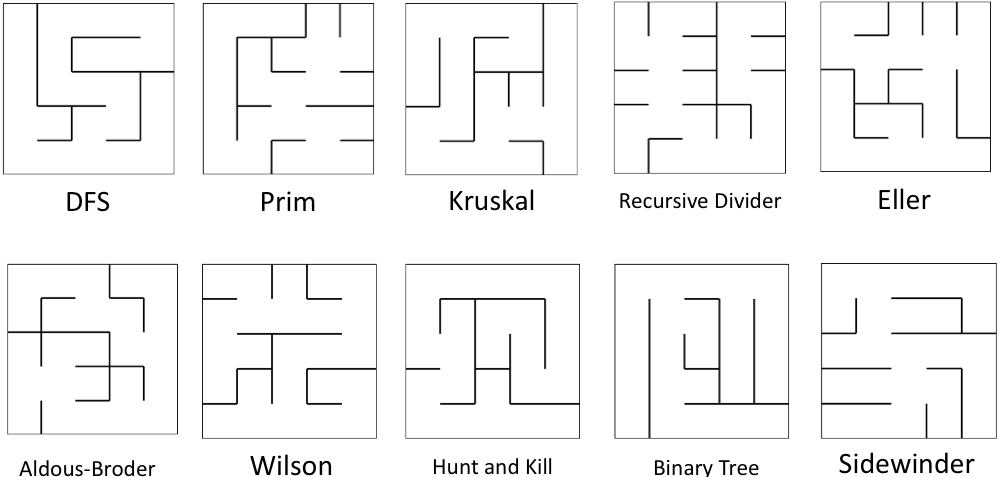
\includegraphics[width=1\textwidth]{images/mazes.png}
\caption{Sample mazes produced by different algorithms.}
\end{figure}


\section{Maze Post-processing}
So far only maze generation has been discussed, however this is not entirely the same as dungeon generation. The mazes that are generated by the maze algorithm have two properties that cause a problem:

\begin{itemize}
\item {\bf Density:} The mazes created are very dense. The term ``density" in a maze refers to the amount of cells that are accessible. In fact, the mazes produced are perfect and hence every cell is accessible from every other cell \citep{ThinkLabyrinth}. However according to Jamis Buck a dungeon will typically be very sparse and have many inaccessible cells \citep{JBuck}.
\item {\bf No loops:} Another property of perfect mazes is that they do not contain any loops \citep{ThinkLabyrinth}, although loops in a dungeon is considered normal \citep{JBuck}.
\end{itemize}

In order to transform the generated mazes into a dungeon-like environment these two properties must be obliterated through some post-process operations.

\subsection{Maze sparseness}
Making the maze more sparse is relatively simple. All that is needed to exclude certain cells from the maze, i.e. we need to wall off these cells completely. However we must insure that walling off a cell does not cause other accessible cells to become inaccessible. In others words, when we wall off a cell we should still end up with a single maze and not multiple independent mazes. Figure \ref{abcd-sparseness} shows an example of a bad implementation of sparseness: walling off cell B cause the cells A, C and D to become separate mazes. We want to insure that this doesn't happen. To avoid this we can simply specify the algorithm to wall off dead-ends only \citep{JBuck}, such as cells A, B or D in Figure \ref{abcd-sparseness}. It's trivial that walling off a dead-end only causes that cell to become inaccessible and doesn't affect any other cells.

\begin{figure}[h!]
\centering
 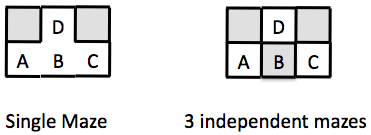
\includegraphics[width=0.38\textwidth]{images/abcd_sparseness.png}
\caption{An example of bad sparseness implementation.}
\label{abcd-sparseness}
\end{figure}

The {\em sparseness factor} defines how many iterations the algorithm should perform. The higher factor will naturally imply a sparser maze \citep{JBuck}. The implementation of this algorithm is expressed as the following (an example of this effect is show in Figure \ref{sparseness2}):

\lstAlgo
\begin{lstlisting}
proc DeadEndRemover(Maze M, Integer Sparseness)
	for I in [1, Sparseness] do
		for each cell C in M do
			if C is a dead-end then
				Wall-off C completely.
			endif
		endfor
	endfor
endproc
\end{lstlisting}

\begin{figure}[h!]
\centering
 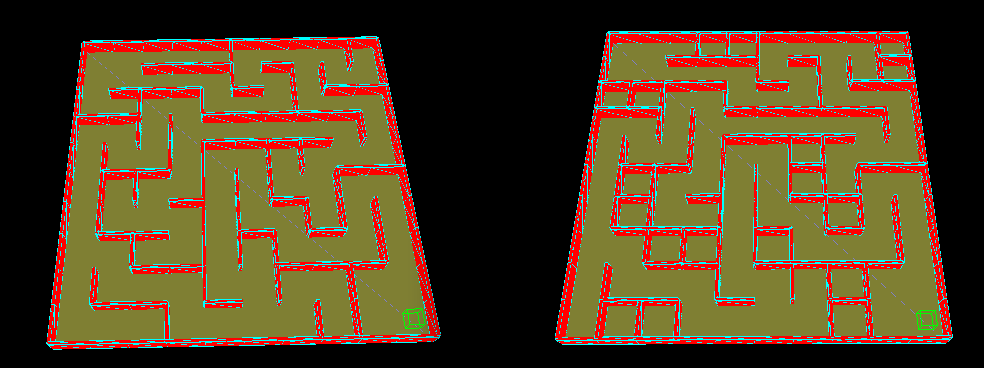
\includegraphics[width=0.74\textwidth]{images/DeadEndDigger-sparse2.png}
\caption{Effect of the dead-end remover with sparseness = 2.}
\label{sparseness2}
\end{figure}

\subsection{Adding loops}
Jamis Buck suggested a method to add loops which should be done after the density-reduction phase. The reason for this is that the concept behind this phase consists of ``restoring" some cells that have been excluded in the previous phase. To create a loop we simple take any remaining dead-end in the maze as a starting point. From this starting point perform a randomised search like with the DFS or Hunt and Kill algorithms. Once we reach a cell which is accessible, (i.e. it has at least 1 wall missing) we stop this search and repeat this process as many times as necessary. Because we break walls until we reach a cell that is part of the maze this causes a loop to be formed \citep{JBuck}.

\begin{figure}[h!]
\centering
 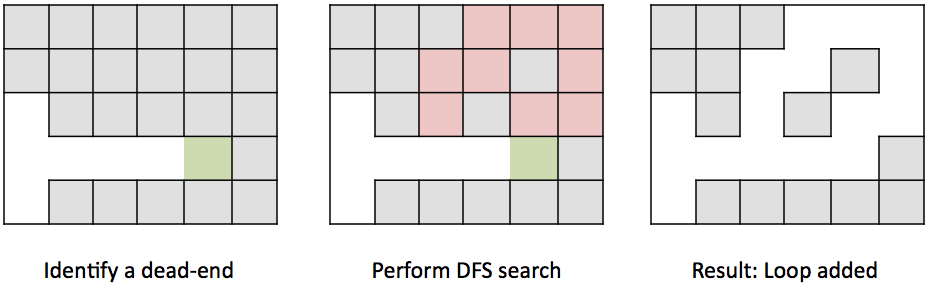
\includegraphics[width=0.74\textwidth]{images/adding_loops.png}
\caption{An example on how to add loops to a maze.}
\end{figure}

However Jamis Buck doesn't not appear to consider cases where the maze doesn't have any dead-ends, which can occur if the sparseness factor is too high. This scenario can be made less frequent by keeping the sparseness factor low but this does not guarantee the presence of dead-ends. There are two possible ways of enforce this phase:
\begin{enumerate}
\item {\bf Add dead-ends:} Before adding loops we could check to see if any dead-ends are present. If not, then we can add random uniformly distributed dead-ends across the maze.
\item {\bf Extending any cell:} We could also modify the original algorithm to start at any random accessible cell and not only dead-ends.
\end{enumerate}

Assuming that dead-ends are present, we can add loops using the following algorithm:
\lstAlgo
\begin{lstlisting}
proc AddLoops(Maze M, Integer NLoops)
	Let I = 0.
	while (I < NLoops) AND (M still has dead-ends) do
		Let C = Random dead-end.
		Let L = The cell that leads into C.
		while C is a dead-end do
			Let D = Step(C, L).
			Let L = C.
			Let C = D.
		endwhile
		Let I = I + 1.
	endwhile
endproc

func Step(Maze M, Cell C, Cell L)
	Let D = a random neighbouring cell of C other than L.
	Break walls between C and D.
	return D.
endfunc
\end{lstlisting}

\subsection{Adding rooms}
The dungeon will often have large rooms that the paths will lead to. Essentially adding rooms involves breaking all the walls in a certain area to open up a lot of space. The rooms themselves represent an empty rectangular area in the maze and can simply be defined by their width and length \citep{JBuck}. One naive approach to first create the dimensions of these rooms then position them anywhere in the maze using a uniform number generator:
\lstAlgo
\begin{lstlisting}
proc AddRooms(Maze M, Integer NRooms)
	for I in [1, NRooms] do
		Pick a random accessible cell C in M.  // use as the top-left
		Pick a random dimension [Width, Length].
		
		// Calculate bottom-right corners.
		Let A = M.GetCell(C.x + Width, C.z + Length).
		
		Break all the walls in between the cells C and A.
	endfor
endproc
\end{lstlisting}

This method is simple and very time efficient. It has a time complexity of $\bigo{n}$ where $n$ is the number of rooms added, which is convenient for very large mazes. However this method will not always give very convincing results because a room is meant to touch as few corridors and other rooms as possible \citep{JBuck}. Jamis Buck suggested a different approach where a {\em weighing system} is used. This consists of testing each possible position for a room and assigning a score to each position. The position with the lowest score is the considered the best solution \citep{JBuck}. The score for a given position and room is calculated using with algorithm:
\lstAlgo
\begin{lstlisting}
func CalcScore(Maze M, Cell Position, Integer RoomWidth, Integer RoomLength)
	Let X0 = Position.x
	Let Z0 = Position.z
	Let Score = 0.
	for I in [X0, RoomWidth] do
		for J in [Z0, RoomLength] do
			Let C = M.GetCell(Position.x + X0, Position.z + Z0)
			if (C is in index range) then
				for each corrider adjacent to C do
					Score = Score + 1.
				endfor
				if C is a corridor then
					Score = Score + 3.
				endif
				if a room is located at C then
					Score = Score + 100.
				endif
			endif
		endfor
	endfor
endfunc
\end{lstlisting}
This method will provide more decent results but it has to iterate over every cell in the maze to find the lowest score \citep{JBuck}. It has a complexity of $\bigo{nm^2}$ where $n$ is the number of rooms and $m$ is the dimension of the maze (assuming the dimension is square).

\begin{figure}[h!]
\centering
 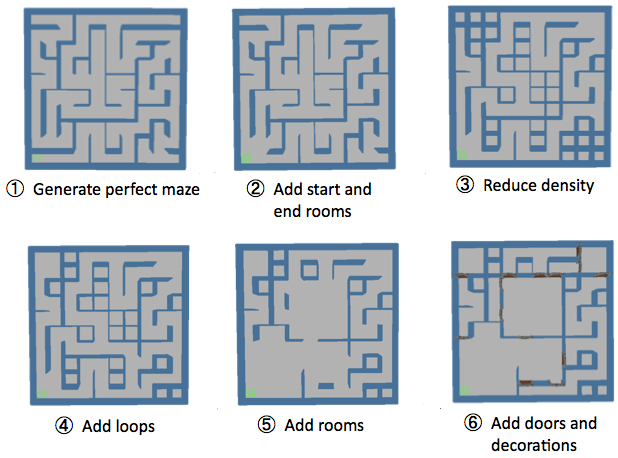
\includegraphics[width=0.8\textwidth]{images/phases-mixed.png}
\caption{The multiple different phases of the dungeon-generation algorithm.}
\end{figure}
\chapter{Mesh and Collider creation}

\section{Mesh Generation}
The maze generation algorithms discussed operate on the classes \texttt{Maze}, \texttt{MazeCell} and \texttt{MazeWall}. However these classes are merely the representation of a mathematical model. In order to use this maze in a 3D environment we need to convert these elements into a 3D mesh. This process is called {\em procedural modelling}. The procedural modelling is carried out by the \texttt{BasicMeshMaker} class with the help of the \texttt{VertexFactory} class. The class creates an array of \texttt{MazeMesh} instances.

\subsection{Procedural modelling}
Procedural modelling is a very difficult task because it essentially involves writing a program that will simulate the human behaviour of a 3D graphics artist. Fortunately, man-made structures such as mazes generally follow a pattern that can be exploited in the modelling process. For instance: walls are designed to be nothing more than a basic cuboid, although detail can always be added to make them look less like a cuboid. Like with many other man-made structures, the floor of the dungeon is intended to be a flat plane.

In order to start procedural modelling, we first need to understand how the 3D plane primitive works because this will be used extensively throughout the algorithm. The plane primitive is composed of 4 corners and 2 triangles (or 1 quad depending on the rendering mode chosen). Divisions can also be added across the plane to increase the polygon count although this is not always necessary.

\begin{figure}[h!]
\centering
 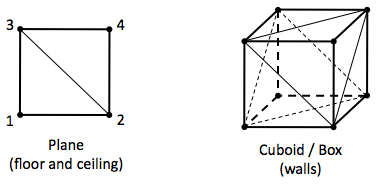
\includegraphics[width=0.52\textwidth]{images/what_is_a_plane.png}
\caption{Vertices and edges of the 3D meshes used to procedurally model the dungeon.}
\end{figure}

The plane can be used as the floor and ceiling of the dungeon to provide a satisfying result. However the plane primitive cannot be used for the walls because this will evidently cause the walls to look far too thin. Therefore we need to use the box primitive for the wall. The box is simply 6 planes stuck to one another.

\subsection{UVW mapping}
Defining the vertex position is not sufficient to produce a good result. In order to render a texture onto the walls and the floor of the dungeon we need to apply a material with a diffuse texture onto those meshes. Each vertex of those meshes will also require a texture coordinate so that the graphics shader can sample the texture for each 3D primitive face.

The question is: how do we define these texture coordinates? Obviously, these coordinates are dependent on the shape of the meshes. For the floor, which we can assume is just a plane, this UVW mapping is very simple to calculate because we can simply map each corner of the plane to its respective corner of the texture. Example: the top-left vertex would map to the UV $(0,0)$, the bottom-right vertex would map to the UV $(1,1)$ and so on.

Using this method will cause the original image to be stretched or squashed if the dimension ratios of the plane and the image don't match. This can be avoided by {\em tiling} the image across the maze cells. Thus we need only to use a square tile texture and maps the corners of the plane to the UV coordinates $(0,0)$ and $(W,L)$, where $W$, and $L$ are width and length of the maze respectively.

For the wall, the procedural UVW mapping is slightly more complicated, although it can be kept simple if we assume that the texture used can be tiled. Because the maps are simply six planes, we can map one face to the texture just like with the floor. However, the face on the opposite side of these coordinates need to be {\em mirrored} so that when two walls are stuck together they will appear as a single wall with a contiguous texture.

\subsection{Adding prefabs}
If we only use planes and boxes to procedurally model our dungeon then the final result will feel very monotonous. This is because we are reusing the exact same shape and texture every time. To reduce the amount of repetition in the dungeon we can add some human-modelled meshes to it to give it more life.

In this project, OBJ files can be imported into the application. However, in order to keep the framework generic, we must not restrain the generator to only using OBJ files. So to keep the framework generic, the generator will simply work with file-names and not the actual mesh. The generator will have no idea what the mesh looks like but will assume that it is scaled, positioned and rotated correctly. Meshes will be placed relative to the walls of the dungeon, so the OBJ files must match these walls. The generator will assume that meshes are facing the front of the scene, scaled to match 1 unit as the length and height of a wall, and positioned such that point $(0,0,0)$ is the centre of the wall's base.

File-names are read from a database and each item is assigned a weight. This weight will allow the user to control the probability of placing specific meshes. Hence, the probability of picking a given item $i$ is:

$$ P(i) = \frac{w_i}{\sum\limits_{j=0}^{n} {w_j} } $$

Where $w_k$ is the weight of the item $k$ and $n$ is the total number of items.

\paragraph{Adding prefabs on the walls}
To decorate the dungeon with assets we can add props such as paintings on the walls. The algorithm that does this simply rolls a dice for each face of each wall (Of course, this ignores the faces that are in-accessible from any part of the dungeon). If the dice roll is above a specified threshold called the {\em density} then a random prefab is selected from the database using the weights to determine their respective probabilities. The use of this {\em density} variable allows the user to control the amount of props that are placed in the dungeon. The dice roll and density are values between 0 and 1. A density of 0 means that no prefabs will be placed at all, 1 means that a prefab will placed on every face. Therefore a density of 0.5 for example will create a dungeon that has prefabs on approximately half of the faces.

\paragraph{Adding doors}
In order to increase the realism of the dungeon it's a good idea to consider adding doors too. To position the doors we need to turn a wall into a door, but we cannot simply place the doors anywhere we want because this might not give a realistic result. There are constraints to consider. For example: placing a door in the middle of an empty space (i.e. no walls around the door) will look pathetic. Doors intuitively lead from one room to another or from a corridor to a room. The constraints that are checked to find potential door candidates are the following:
\begin{itemize}
\item {\bf Only consider walls that don't exist:} This constraint is used to avoid breaking the wall of an inaccessible cell, because this would cause the door to lead to a single-cell (i.e. a dead-end).
\item {\bf Insure the walls on the sides of the door exist:} If the door doesn't have walls on the sides then the players can simply walk around them. This type of door is particularly useless and should be avoided.
\item {\bf The door must lead to atleast one room:} As discussed, doors intuitively lead to a room. A room can be considered as any empty space of minimum size 2x2. Needless to say, this room should be adjacent to the door.
\end{itemize}

Other than checking for these specific constraints, the process of placing doors is identical to that of placing items on the walls themselves. Adding these prefab models to the dungeon greatly enhances the overall aesthetic of it. Unfortunately, if the library of prefabs used is not sufficiently large then many objects will reappear repeatedly. Therefore a very large library is required in order for this method to be efficient.








\section{Colliders used}
The interactions between the player and the dungeon are often very game-specific, thus we cannot generalise this. However, collision detection and response is a feature that is probably common amongst all 3D video games. Therefore this aspect is more or less compulsory to implement in a generic framework.

To test if one mesh $M_1$ is colliding with another mesh $M_2$, the perfect collision detection algorithm checks if any triangle of $M_1$ is colliding with any triangle of $M_2$. Although computers are fast, this brute-force method will quickly get very expensive for high-polygon meshes and as the number of meshes in the scene increases \citep{BVH}. In a real-time applications, this method is not acceptable and either an optimisation or an approximation must be used.

A typical form of optimisation is to use a bounding volume to test for collision detection. This consists of using a primitive shape such as a sphere or a box to approximate the area of mesh. Because of the mathematical simplicity of these primitives we can perform collision tests very quickly with a complexity of $\bigo{1}$ \citep{BVH}. Some common bounding volumes include the following:
\begin{itemize}
\item {\bf Bounding Sphere:} This consists simply of a {\em radius} and {\em centre}. This is the cheapest type of bounding volume but is generally quite in-accurate.
\item {\bf Axis-Aligned Bounding Box (AABB):} This is cuboid with a {\em width}, {\em length} and {\em height} (or simply a {\em volume}) along with its {\em centre}. The box always remains aligned with the $xyz$-axes of the world space.
\item {\bf Oriented Bounding Box (OBB):} Like the AABB, the OBB also has a volume and centre. However, it also has an {\em orientation} component, making it more accurate but also more expensive.
\item {\bf Bounding Frustum:} This bounding volume is typically used in frustum culling to check if an object is in the view-port of the camera.
\end{itemize}

We need to construct a bounding volume for each individual wall. In the dungeon, the walls are all aligned with the $xyz$-axes and are all box-like shapes. This makes the AABB an ideal candidate because it will provide very fast and extremely accurate results. For this reason the AABB volume will be exploited to the fullest potential. Nevertheless, this will restraint the dungeon to only being allowed to rotate 90\degree, although this is not a deal big because an AABB can be considered as an OBB with an orientation of 0\degree on each axis. Therefore extending the framework to support orientation would not be complicated.

To calculate the AABB we can use variables defined in the \texttt{Maze} class. To calculate the centre of the box we need the cell width $W$ and length $L$, the height of the wall $H$ and the indices $(i_x, i_z)$ of the wall:
\begin{itemize}
\item {\bf For vertical walls:} $(x,\,y,\,z)= (i_{x}W,\, \frac{H}{2},\, i_{z}L+\frac{L}{2})$
\item {\bf For horizontal walls:} $(x,\,y,\,z)= (i_{x}W+\frac{W}{2},\, \frac{H}{2} ,\, i_{z}L)$
\end{itemize}
To calculate the volumes, we can use the values of $W$, $L$ and $H$ directly along with the thickness of the walls $T$:
\begin{itemize}
\item {\bf For vertical walls:} $(w,\,h,\,l)= (T,\, H,\, L)$
\item {\bf For horizontal walls:} $(w,\,h,\,l)= (W,\, H,\, T)$
\end{itemize}

\subsection{Bounding Volume Hierarchy}
Despite the fact that bounding boxes are very time-efficient they remain very expensive once the mesh count in the scene is high. If the scene is composed of millions of bounding boxes then the testing phase will require a significant amount of time and drop the frame rate to an unacceptable level \citep{BVH}. The number of AABBs contained in our maze is of order $\bigo{xz}$ where $(x,z)$ is the dimension of the maze, and in the worst case where $x=z$ we get a quadratic complexity $\bigo{x^2}$. For example, a maze of dimension $(100,100)$ will have upto $20 000$ boxes. Therefore, an extra optimisation is absolutely mandatory in order for the framework to support applications that require a large scale maze.

\subsubsection{Theory}
One very efficient method to test for collisions amongst a large set of colliders is to use a Bounding Volume Hierarchy (BVH). The idea behind the BVH is to categorise the colliders into groups and sub-groups to quickly identify which colliders could be potentially colliding and which ones are definitely not colliding. The BVH structure divides the colliders in the form of a tree. The brute method of testing for collision with each individual collider has a complexity $\bigo{n}$, where $n$ is the total number of colliders. The BVH aims at turning this linear complexity into a logarithmic one: $\bigo{\log_{k}n}$ where $k$ is the number of children per parent node in the tree \citep{BVH}. 

All the leaf nodes are the colliders themselves that are used to determine whether a collision is occurring or not. Whereas the parent node contains a collider that encapsulates all of its children. When checking the collisions the upper nodes in the tree are tested first starting with the root. If a parent collides then the algorithm recursively checks the children. However if a parent doesn't collide then the children do not need to be tested, thus eliminating a large number of tests and speeding up the collision detection \citep{BVH}.

\subsubsection{Dividing the maze}
To construct a BVH for the maze that contains the colliders of the walls and the floor we can recursively divide the maze into four sections (top-left, top-right, bottom-left, bottom-right) until we reach the individual maze cells.

\begin{figure}[h!]
\centering
 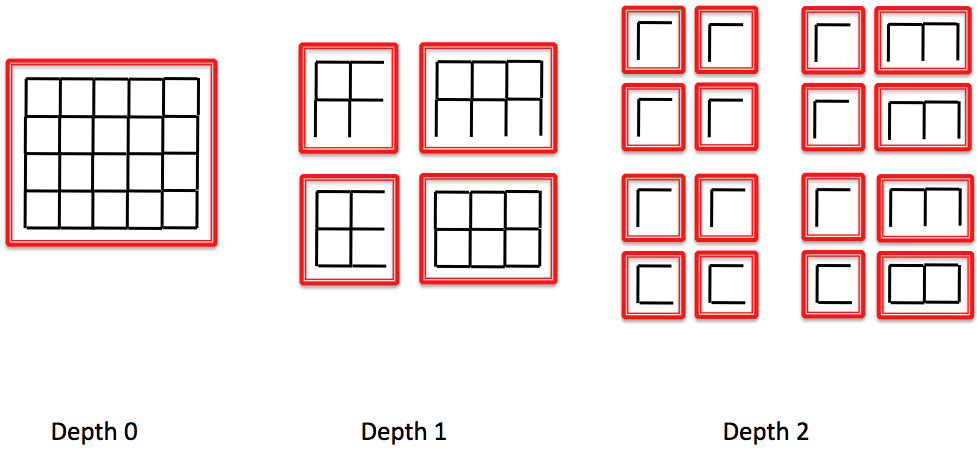
\includegraphics[width=0.74\textwidth]{images/bvh_maze.png}
\caption{An example of a BVH for a maze of dimension (5, 4). The red boxes represent parent nodes at a specific depth of the tree. The black lines represent the colliders of the walls.}
\end{figure}

However there are a few things to keep in mind:
\begin{enumerate}
\item {\bf The walls are shared amongst cells:} Although $k=4$ is used to sub-divide the maze we should avoid having the same collider stored twice in the BVH because this is an un-necessary waste of time and space. Therefore, when we reach the deepest parent nodes we should only have 2 children nodes: one for the top wall and another for the left wall.
\item {\bf There are more walls on the edge:} If we use the convention mentioned above then this would exclude all the walls on the very right and bottom edge of the maze. The nodes on those borders will need to have 3 or 4 children instead of 2.
\item {\bf Odd number division:} If a dimension is odd, then the bottom or right sections should be made slightly bigger to absorb the division's remainder and avoid colliders from getting excluded.
\end{enumerate}

The algorithm for constructing this BVH is given by:

\pagebreak
\lstAlgo
\begin{lstlisting}
func ConstructBVH(Maze M)
	Let C0 = cell number (0,0).
	Let C1 = cell number (M.Width-1, M.Length-1).
	Let R = ConstructNode(M, C0, C1).
	return a new BVH with root R.
endfunc

func ConstructNode(Maze M, Cell From, Cell To) // recursive
	Let R = a new BVH node.

	if From == To then
		Let L = Empty set {}.
		Calculate colliders of top and left walls. Add those to L.
		if To.X == Width-1  then add right wall to L as well. endif
		if To.Y == Height-1 then add bottom wall to L as well. endif
		Make L the children of R.
	else
		// Divide From-To into 4 spaces:
        /**
         *   +----+----+
         *   | S1 | S2 |
         *   +----+----+
         *   | S3 | S4 |
         *   +----+----+
         */
         foreach Non-empty space S in {S1, S2, S3, S4} do
         	Let C = ConstructNode(M, S.From, S.To).
         	Make C and child of R.
         endfor
	endif
	
	Calculate Bounding-box of R.
	return R.
endfunc
\end{lstlisting}
\chapter{Software design and structure}
With the theory of mazes and random number generation thoroughly briefed we can now explore the implementation of these algorithms. The software has a high level of abstraction and is designed to maximise code re-usability. It was developed in C++ and OpenGL; it is ported on both Mac OS X and Windows which further encourages code re-usability. Despite being implemented using OpenGL, the generator itself remains fully independent from OpenGL and can even be re-used with a different graphics library such as Microsoft's DirectX.

{\em DunGen} is the name of the software that was produced in parallel to the research. The software is designed as an extendible framework for dungeon generation. It implements most of the techniques discussed regarding maze and dungeon generation. It also contains a sample application in which a green wire-framed cube can be moved by the user and collide with the walls of the maze. All the source code is found in the {\em src} directory.

See appendix \ref{screenshots} for screen-shots of the final product and appendix \ref{codeDiagrams} for code listings and class diagrams

\section{The Engine}
The Generator is intended to be engine-independent. However, for the purpose of demonstration, a small engine was developed. The software runs using OpenGL and the math library GLM although it is possible to port the code to use other libraries. The engine used in the software is very primitive because it is only meant to be used to render the maze, handle axis-aligned bounding box (AABB) collisions and listen to user-input.

\paragraph{Features}
The features of the engine are found in the following directories:
\begin{itemize}
\item {\bf Engine/Core/Application/} Contains classes regarding argument-parsing and starting/exiting the application.
\item {\bf Engine/Core/File/} Used for handling files on different platforms.
\item {\bf Engine/Core/Timing/} Keeps track of timing in a static class.
\item {\bf Engine/Graphics/Camera/} The camera class containing values for {\em pitch}, {\em yaw}, {\em roll}, {\em field-of-view}, {\em near-clip-plane} and {\em far-clip-plane}.
\item {\bf Engine/Graphics/GraphicsContext/} Controls graphics context. GLFW is used to manage this on different platforms.
\item {\bf Engine/Graphics/Material/} Class describing the material of a 3D object.
\item {\bf Engine/Graphics/Mesh/} The Mesh class containing vertex positions, UVW co-ordinates and primitive indices.
\item {\bf Engine/Graphics/Renderer/} The class used to render the content of the scene.
\item {\bf Engine/Graphics/Texture/} Image bitmap handling, used by Mesh instances to diffuse a texture. The library SOIL is used to load PNG files.
\item {\bf Engine/Input/} Contains classes to examine keyboard and mouse states.
\item {\bf Engine/Scene/} Contains classes to control the content of the scene.
\item {\bf Engine/Tools/} Math functionalities.
\end{itemize}

\section{The Generator}

\subsection{The Maze}
The maze can be viewed as a static graph. It is composed of vertices (called cells) and edges (called walls); hence there are 3 classes used to represent the maze:
\begin{itemize}
\item \texttt{Maze}: The maze itself. It contains all the maze-cells and walls within an array. It also contains several queries and operations that can be used by a multitude of algorithms.
\item \texttt{MazeCell}: This class represents a single cell. It contains a {\em visited} field because this is essential for maze generators. It also contains its $x$ and $y$ co-ordinates to make it fast and simple to know where the cell is situated.
\item \texttt{MazeWall}: This class represents either a vertical or horizontal wall. It can be either of type 
\texttt{MAZE\_WALLTYPE\_NONE} (no wall) or \texttt{MAZE\_WALLTYPE\_DEFAULT} (there is a wall), this domain can easily be extended to support different types of walls, such as doors for instance.
\end{itemize}

\subsection{Graph Implementation}

There are multiple different structures that implement the graph data structure. Each one has its advantages and disadvantages. M. Goodrich and R. Tamassia have listed a number of possible suggestions in their book {\em  Data Structures And Algorithms in Java} \citep{DSAJ-4}.
\begin{itemize}
\item {\bf Adjacency List:} In this data structure, the vertices are stored in a linked list. Each vertex also stores a list of adjacent vertices. This structure is optimised for adding and removing edges or vertices very fast with a complexity of $\bigo{1}$ \citep{DSAJ-4}.
\item {\bf Incident List:} Very similar to the adjacency list structure, however incident rays are also stored in a list. Likewise, this structure is optimised for adding and removing elements of the graph \citep{DSAJ-4}.
\item {\bf Adjacency Matrix:} In this structure data of adjacent vertices is stored in a 2D array. This method is not very memory efficient for sparse graphs and is very slow at adding or removing vertices (complexity $\bigo{V^2}$). One big advantage though is that this structure has a complexity of $\bigo{1}$ for queries, making it ideal for static dense graphs \citep{DSAJ-4}.
\end{itemize}

In order to implement the maze, a data structure similar to that of the adjacency matrix was chosen. However the elements of the matrix store the vertices (cells) themselves and not the adjacent vertices. The reason for this is that the maze's dimension is completely static and the adjacent vertices are pre-defined. The dimension of the maze is only specified once at the initialisation and cells are never removed. In contrast to arrays, lists are optimised for dynamic structures that require frequent adding and removal, which is entirely unnecessary in this case and hence arrays are favourable \citep{DSAJ-4}. 

Arrays provide the advantage of direct access through the use of an index. This is exceptionally useful because cell query operations are very frequent in the algorithms that we have observed in the previous chapters. The cells are stored in a single dimensional array to keep memory contiguous but this array is used as a two-dimensional array. The 1D index of a cell $(x,y)$ in a 2D space can be calculated by the formula:
$$ I_{cell}(x,y) = x + yW \;\;\;\;\;\; \text{where }W=\text{width of the maze} $$

As mentioned previously, the incident edges do not need to be stored because given a cell $(x, y)$, we know that this cell has 4 adjacent nodes: $(x+1,y)$, $(x-1,y)$, $(x,y+1)$ and $(x,y-1)$ (assuming that $(x, y)$ isn't a borderline cell). However, data about the walls still needs to be stored somewhere. This is stored in an array for same reasons the that cells are. Vertical and horizontal walls are stored in separate arrays; the reason for this is the two arrays are of different dimensions. In mathematical terms
\begin{itemize}
\item Let $W=$ the number of cells along the $x$-axis.
\item Let $L=$ the number of cells along the $y$-axis.
\item The dimension of the vertical wall array is $(W+1,L)$.
\item The dimension of the horizontal wall array is $(W,L+1)$.
\end{itemize}

\subsection{Random Number Implementation}
All the algorithms have some kind of randomness within them. The randomness in these algorithms remains abstract and changing the behaviour of how random elements are chosen can effect the outcome of the dungeon, much like how the Growing Tree algorithm can generate different types of mazes based on how the random selection works \citep{ThinkLabyrinth}.

Concerning random number generation in PCG something simple such as a LCG will suffice. LCGs are not cryptographically secure but this is not an issue because there is no need to hide anything. Additionally LCGs provide the advantage of being fast and reproducible. So if we do not want to store a generated dungeon because of memory concerns then we can simply store the seed and run the algorithm again to restore the old dungeon. Needless to say, research has shown that we need good parameters to obtain numbers that are statistically adequate. Finding a good LCG is a difficult task, so instead we will simply use the one suggested by Park and Miller because that one has a large amount of evidence supporting its reliability. Reminder: The coefficients of this LCG are $M = 2^{31}-1$, $a = 7^5$ and $c = 0$. Normally on the lower-order bits would have to left un-used because they produce bad results, however this is not necessary in this case because the modulus in not of the form $2^i$ \citep{park_miller}.

For the most part, we can simply used an integer generator with a uniform distribution. Random elements can be picked from a set by generating a random index within range. However in some cases we might need a non-uniform distribution. For instance, let us consider the DFS maze generation algorithm. If a uniform number generator is used then the algorithm will have an equal chance to turn right, to turn left or carry on straight. This means that the probability of carrying on straight is $\frac{1}{3}$ and the probability of turning is $\frac{2}{3}$ (assuming that all 3 options are available), which will trivially cause lots of turns to occur. If we want to reduce this we can use the class {\tt RandomTurner} in the framework. This class uses a random-float generator to produce integers such that the probabilities of turning left, right or going straight are different. This is useful if we want to use a DFS or Hunt-And-Kill generator that turns less often.

The number generators can be found in the {\em Generator/Random/} directory. It consists of 2 interfaces:

\begin{enumerate}
\item {\bf RandomI:} This interface defines a random {\em Integer} generator.
\item {\bf RandomF:} This interface defines a random {\em Floating-point} generator.
\end{enumerate}

There is 1 class implementing both of these interfaces and 1 implementing only the \texttt{RandomI} interface. Respectively, these classes are:
\begin{enumerate}
\item {\bf UniformRandom:} This class produces random integers and floats that follow a uniform distribution. It uses a 32-bit LCG to produce these numbers.
\item {\bf RandomTurner:} This class is used by maze generators such as the depth-first search generator to allow more control over the probability of turning. It produces random integers between 0 and 2 using a \texttt{UniformRandom} instance and given probabilities.
\end{enumerate}

\subsection{Diggers}
At this stage, the dungeon generation algorithm is divided into a sequence of phases. Generating a dungeon consists of generating a maze and then applying some post-processing actions on it \citep{JBuck}:
\begin{enumerate}
\item Generate a maze.
\item Reduce density of maze.
\item Add loops in the maze.
\item Add rooms in the maze.
\end{enumerate}
\begin{figure}[h!]
\centering
 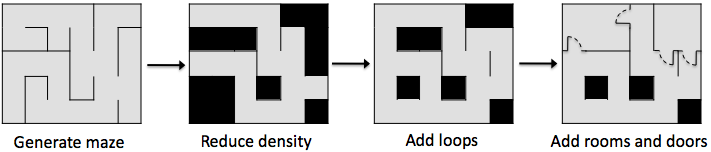
\includegraphics[width=0.66\textwidth]{images/makeDungeon4steps.png}
\caption{The 4 major steps to generate a dungeon.}
\end{figure}

If we interchange, remove or modify these phases we will obtain different result. Ideally, to keep the framework as generic as possible, the user should have full access to any of these phases and should be allowed to use them in whichever order they please to. To allow this kind of freedom to the user the DunGen framework will be based around these phases. Each phase will be referred to as a {\em Digger} and will alter the shape of the maze in some way.

All the diggers in the application extend the abstract \texttt{Digger} class that contains the initialisation, iteration and ending steps of the algorithm. Each digger implements the \texttt{Step} function (along with other functions) that corresponds to a single step in the algorithm. This function returns \texttt{true} once the looping is complete. To run a digger we need only to call the \texttt{DigFully} function that runs all these steps.
\lstCpp
\begin{lstlisting}
void Digger::DigFully()
{
	Init();
	while(!Step());
	End();
}
\end{lstlisting}

\paragraph{DFSDigger} This digger generates a maze using the DFS algorithm. The algorithm is implemented using a back-tracking stack\footnote{Actually a \texttt{std::list} is used, but it is used as a stack}. Every-time the algorithm visits a new node with more than one child it adds this node to the stack. Whenever it visits a new node with no children it backtracks by popping a node from the stack and carries on from there.
\paragraph{PrimDigger} This digger generates a maze using Prim's maze generation algorithm. It is implemented in a similar way to the Depth-first search digger, except that it uses a list instead of using a stack. The algorithm always adds newly visited nodes to the list and removes them when they no longer have any unvisited children. At the start of each iteration, a random node from this list is chosen.
\paragraph{KruskalDigger} Another digger used to generate a maze using Kruskal's algorithm. The algorithm is implemented with the use of the helper classes \texttt {KruskalEdge} and \texttt{SpanningTree} to quickly identify whether or not 2 cells belong to the same spanning tree.
\paragraph{BinaryTreeDigger} This digger generates a maze using the binary-tree maze generation algorithm. This digger simply removes either the top or left wall for each cell in the maze. However, it insures not to remove any walls at the extreme edges of the maze.
\paragraph{StartEndDigger} This digger simply creates a small 2x2 room on the top-left and bottom-right corners. This digger can be placed before the \texttt{DeadEndDigger} to prevent that digger from leaving the player in a 1x1 room.
\paragraph{DeadEndDigger} This digger increases the sparseness factor of a maze by walling off dead-ends. The {\em sparseness} factor defines the number of iterations to perform. On each iteration the digger finds all the dead-ends in the maze and walls them off.
\paragraph{LoopDigger} This digger uses a random float generator and a given probability to determine which dead-ends should be turned into loops. It uses a randomized walk similar to that in Wilson's algorithm \citep{DBLP:conf/stoc/Wilson96}.
\paragraph{RoomDigger} This digger places random rooms at any random positions in the dungeon. It simply breaks walls at random areas and doesn't check for any constraints.
\paragraph{WeighedRoomDigger} This digger, like the \texttt{RoomDigger}, also places random rooms across the dungeon. However, this digger uses a weighing system to find the best suitable way to place the rooms \citep{JBuck}.
\paragraph{WallDecoDigger} This digger randomly places external 3D meshes onto the walls. It provides file-names, translation and rotation that can be used by the engine to load the meshes.
\paragraph{DoorDecoDigger} Identical to the \texttt{WallDecoDigger}, but for the doors.

\section{Launcher}
The DunGen software comes with a Launcher developed in Java. This Launcher is designed to make it easy to quickly parametrise the dungeon generator and launch it. The Launcher is very useful to analyse how the dungeons created vary according to the parameters used. Number generators and diggers can be added, removed and configured as the user wants. The properties of the number generators and diggers are exported by the Launcher into a {\em .dungenprofile} file that is read by the DunGen program.

The user can specify which texture files to use to display the dungeon along with the random seed and maze dimension. Minimal graphics options are also available to the user. The launcher runs the DunGen program as a child process and displays the program output stream in a text-area.

All the source code of the DunGen launcher can be found in the {\em Projects/eclipse/Launcher/src/} directory. See appendix for screen-shots.

\begin{figure}[h!]
\centering
 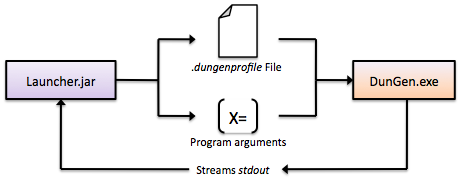
\includegraphics[width=0.52\textwidth]{images/launcherAndDungen.png}
\caption{Interaction between the Launcher and the DunGen program.}
\end{figure}
\chapter{Conclusion}

Based on the research that was carried out is it clear now that procedural content generation (PCG) is a vast and very complicated field in computer science. We have observed a number of different techniques that can be used to generate content, each with their advantages and disadvantages. Amongst all these techniques are there is no single best PCG algorithm. Every content generator generally focuses on a particular type of environment and so a different technique should be used depending on the desired result. For example, using a search-based or rhythm-based method to generate mountains is probably not the best approach. Because of this, picking what kind of algorithm to use and how to implement it is very crucial.

To generate random content, one must have access to some sort of random elements. The randomness of the content is moderated through the use of random integers and floating-point numbers. Getting access to pure random numbers, meaning numbers that are truly random, is not really possible in computing. Instead, we use random number generators that create pseudo-random numbers. These numbers are entirely deterministic (apart from the time-based seed) but, if good parameters are used, they will have a distribution that appears to be random \citep{yu_random}.

Pseudo-random number generators including the Coupled Congruential Generator, the Mersenne Twister and the Blum Blum Shub are suitable in the field of cryptography. However cryptographically secure number generators are not required in simulations and therefore Linear Congruential Generators (LCG) are generally good enough for the use of procedural content generation. 

Finding and picking out a good LCG is an exceptionally difficult task to manoeuvre around. LCGs require a period that is as long as possible because those with a short period have historically caused a few issues. Large word-sizes for the modulo must be used along with other constraints in order to guarantee this long period. However a LCG with long period will not necessary provide good results. Statistical tests need to be performed on a LCG to insure that it produces numbers with adequate statistical randomness. Many different LCGs were examined in order to chose a satisfying number generator.

In addition to a good number generator, generating content requires the help of a solid and well-detailed mathematical model describing the patterns of the environment as closely as possible. These models vary tremendously for different types of environments and can be very difficult to conceptualise due to their complexity. For instance, to generate mountain-like environment Perlin noise can be used to generate a random height-map. Multiple random sine waves can also be used to generate a wavy height-map of a 2D game. Rhythm-based approaches can be used whenever timing is a crucial factor, such as 2D side-scroll platform games \citep{DBLP:journals/tciaig/SmithWMTMC11}. 

The model used to generate a dungeon-like environment is merely a tangent of maze generation. Mazes on their own already have a very elaborate theory established. Properties such as perfection, sparseness, biased and river are rigorously defined. There are multiple different algorithms that can be used to generate a perfect maze. Some of these algorithms are very similar to one another, such as the Depth-first search and Hunt-and-Kill algorithms, the Aldous-Broder and Wilson's algorithm, or the Binary-tree and Sidewinder. On the other hand some algorithms, such as the Recursive Division algorithm, are entirely different to all other algorithms. All these different algorithms have all been conceived in such a way that they all generate perfect mazes, however they all produce different types of mazes that can look very distinctive to one another.

Because of this wide variety of maze generators, picking which one to use is not obvious. The depth-first search and Hunt-and-Kill algorithm both have a large river factor which makes generally makes them produce more satisfying results \citep{JBuck}. However, algorithms like the Binary-tree algorithm are highly biased \citep{ThinkLabyrinth} which can potentially make them useful to one who wants to generate a dungeon that targets a specific direction.

Generating a basic mesh for the maze is not too complicated if we simply use 3D boxes to model the walls and tiled-textures for the UV mapping. From a programming perspective this is an efficient way to procedurally model the dungeon. But from an aesthetic point of view the result is not very satisfying. The aesthetic can be improved upon by using an occupancy-based algorithm; the method chosen consists of adding 3D meshes that are modelled by humans.

Despite the efforts, there is too much repetition and the dungeon looks similar almost everywhere. This is one of the major problems with PCG which was discussed very early on. PCG simply cannot produce levels that are unique. Even though levels are generated with different seeds and may look different they will still have obvious similarities. Some things can be done to reduce the repetition effect but it can never be blotted out completely. For instance, occupancy allows level designers to make specific parts of level look unique but chunks can still be re-used in several levels or within a level itself.

Overall we noticed that creating a generic framework for content generation is not simple because the possibilities are only limited to the imagination of designers. The algorithm used in the developed framework is essentially completely blank at the start and it is up to the user to define precisely how it should behave. There is an apparent reason for this: as specific details and constraints are added to desired result the generator's algorithm become increasingly more complex. In fact a slight change in the specification of the desired result can have a major impact on the algorithm used. Therefore resorting to a game-specific algorithm  might not always be a bad idea and this is probably why most game-developers focus on this.

\pagebreak
\addcontentsline{toc}{chapter}{Bibliography}
\bibliographystyle{apalike}
\bibliography{MyBib}

\pagebreak
\appendix
\chapter{Screen-shots}
\label{screenshots}

\begin{figure}[h!]
\centering
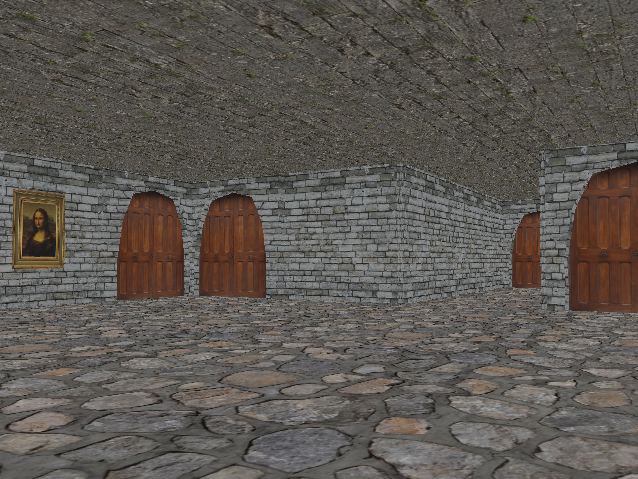
\includegraphics[width=0.49\textwidth]{images/dungeon02.png}
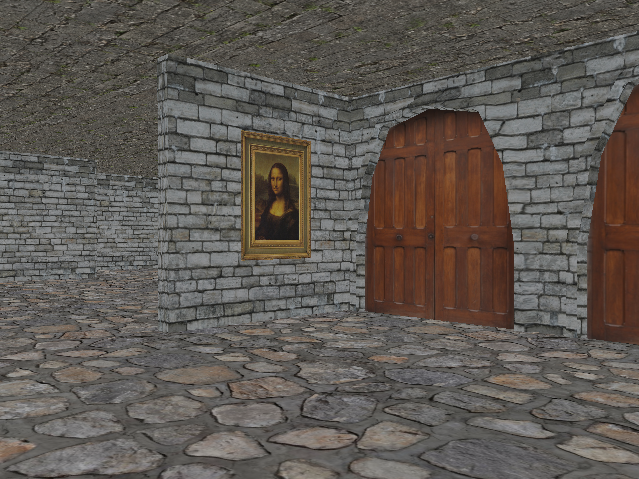
\includegraphics[width=0.49\textwidth]{images/dungeon03.png}
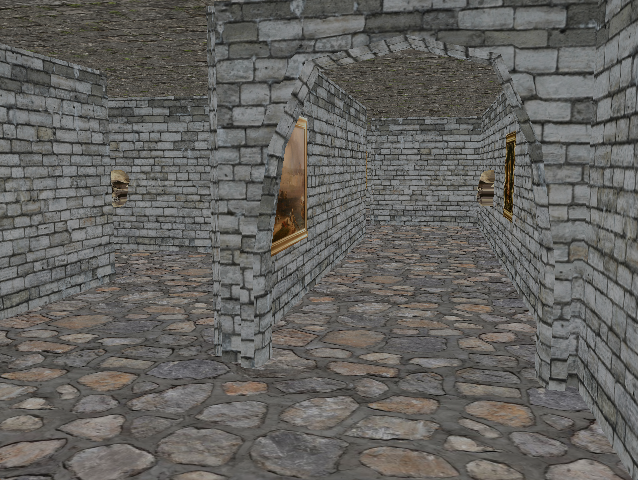
\includegraphics[width=0.49\textwidth]{images/dungeon04.png}
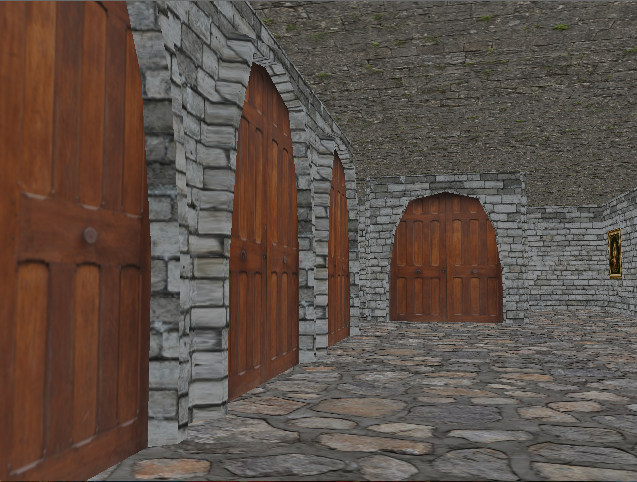
\includegraphics[width=0.49\textwidth]{images/dungeon05.png}
\caption{Screen-shots of the final result.}
\end{figure}

\begin{figure}[h!]
\centering
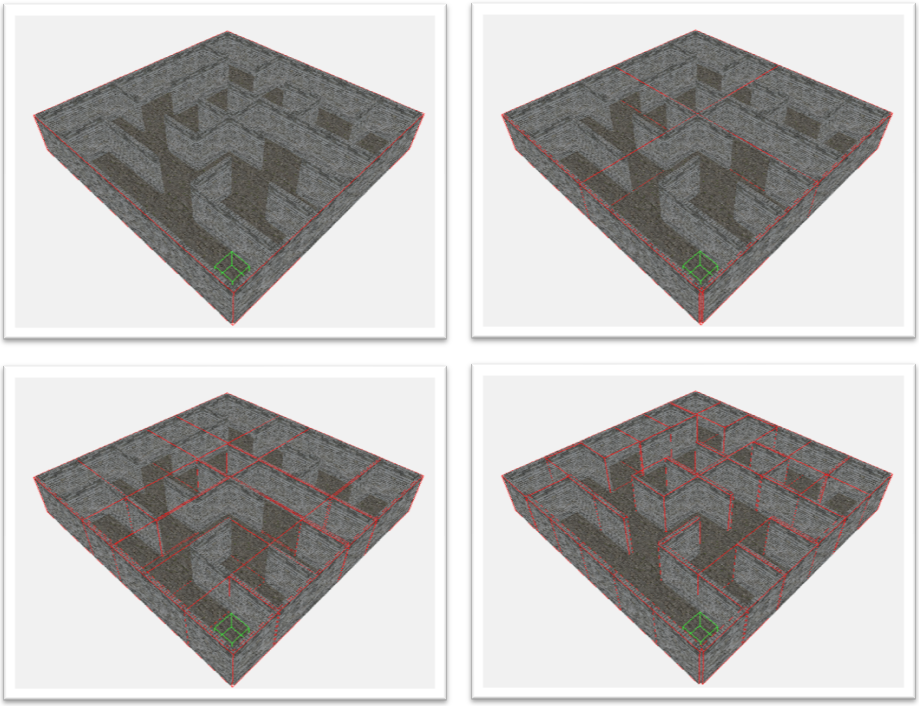
\includegraphics[width=1\textwidth]{images/bvh-depths.png}
\caption{Screen-shots of the BVH at different depths.}
\end{figure}

\begin{figure}[h!]
\centering
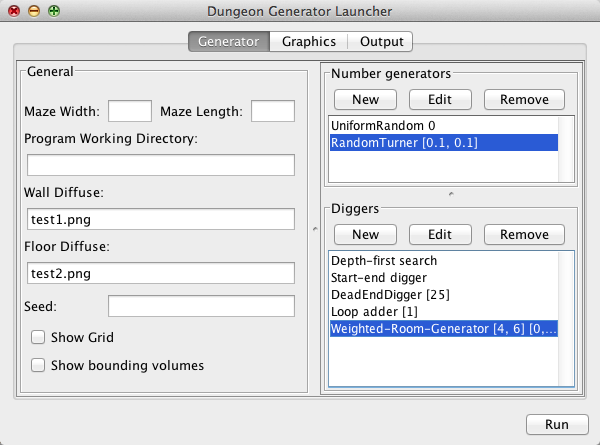
\includegraphics[width=0.49\textwidth]{images/launcher00.png}
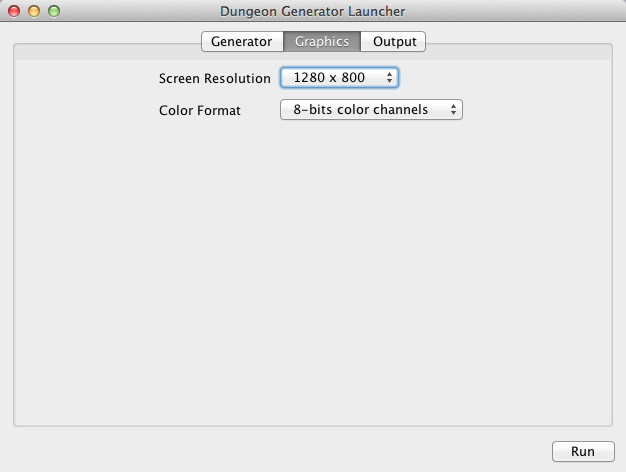
\includegraphics[width=0.49\textwidth]{images/launcher01.png}
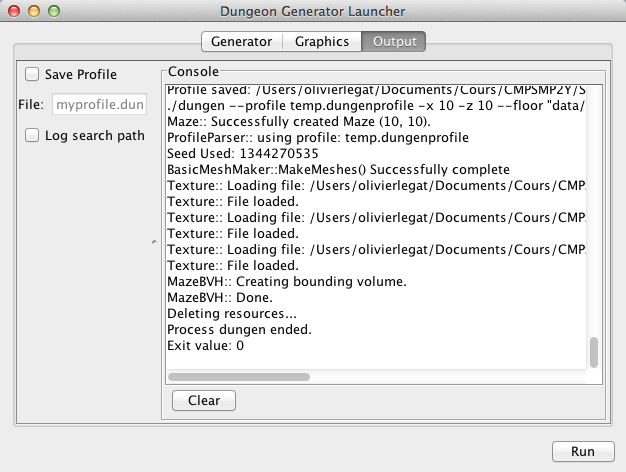
\includegraphics[width=0.49\textwidth]{images/launcher02.png}
\caption{Screen-shots of the launcher.}
\end{figure}








\chapter{Code and Class Diagrams}
\label{codeDiagrams}

\section{Class Diagrams}
\subsection{DunGen}
\begin{figure}[h!]
\centering
 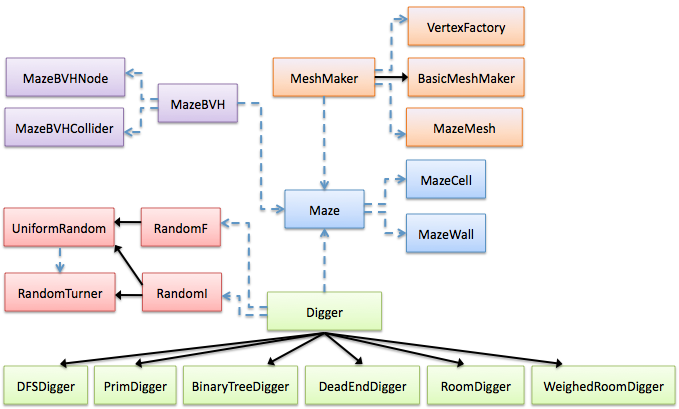
\includegraphics[width=0.80\textwidth]{images/uml_generator0.png}
\caption{Class diagram of the generator structure.}
\end{figure}

\pagebreak
\begin{figure}[h!]
\centering
 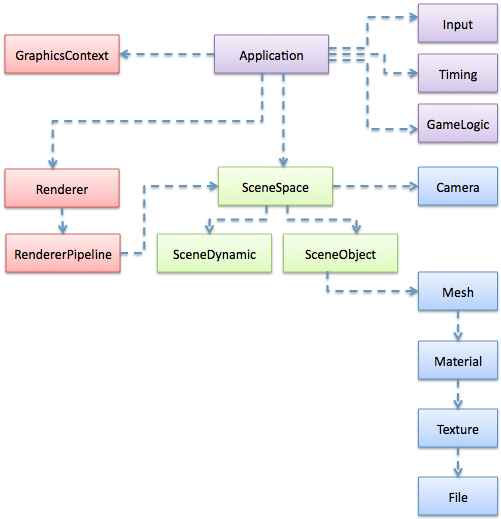
\includegraphics[width=0.65\textwidth]{images/uml_engine0.png}
\caption{Class diagram of the engine structure.}
\end{figure}

\pagebreak
\subsection{Launcher}
\begin{figure}[h!]
\centering
 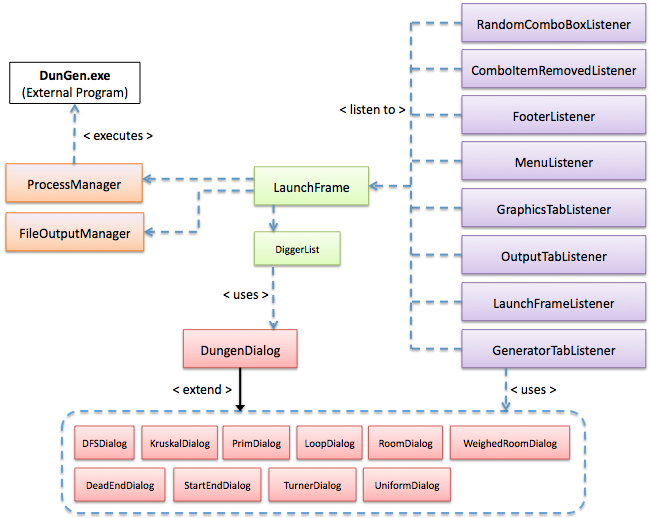
\includegraphics[width=0.78\textwidth]{images/uml_launcher0.png}
\caption{Class diagram of the launcher's structure.}
\end{figure}


\section{Code Listings}
The code listing in this appendix does not cover all the code of project. Only the critical sections that are discussed thoroughly in the dissertation are displayed here.

\subsection {Maze cells and walls}
\lstCpp
\begin{lstlisting}[caption= The \texttt{MazeCell} class]
enum MazeCellType
{
    MAZE_CELL_WALL,
    MAZE_CELL_FLOOR
};

class MazeCell
{
public:
    MazeCell(int x, int z, MazeCellType type);
    ~MazeCell();
    
    bool IsVisited() const {return visited;}
    void SetVisited(const bool b) {visited = b;}
    
    MazeCellType GetCellType() const {return type;}
    void SetCellType(MazeCellType celltype) {type = celltype;}
    
    int X() const {return x;}
    int Z() const {return z;}
    
    Object* GetObject() const {return obj;}
    void SetObject(Object* o) {this->obj = o;}
    
private:
    int x, z;
    MazeCellType type;
    bool visited;
    Object* obj;
};
\end{lstlisting}

\lstCpp
\begin{lstlisting}[caption= The \texttt{MazeWall} class]
enum MazeWallType
{
    MAZE_WALLTYPE_NONE,
    MAZE_WALLTYPE_DEFAULT
};

enum MazeWallPosition
{
    MAZE_WALLPOS_UP,
    MAZE_WALLPOS_DOWN,
    MAZE_WALLPOS_LEFT,
    MAZE_WALLPOS_RIGHT
};

class MazeWall
{
public:
    MazeWall();
    ~MazeWall();
    
    MazeWallType GetType() const { return type; }
    void SetType(MazeWallType t) {type = t;}
    
private:
    MazeWallType type;
};
\end{lstlisting}

\subsection {Maze}
\lstCpp
\begin{lstlisting}[caption= The \texttt{Maze} class]
class Maze
{
public:
    Maze(int width, int length);
    ~Maze();
    
    /**
     * Get a cell.
     * @param A pointer to cell. If [x,z] is out of range, NULL is returned.
     */
    MazeCell* GetCell(const int x, const int z) const;
    MazeWall* GetWall(const MazeCell* cell, MazeWallPosition pos) const;
    MazeWall* GetWall(const int x, const int z, MazeWallPosition pos) const;
    
    MazeWall* GetVWall(const int x, const int z) const {return vwalls[x + z * (width+1)];};
    MazeWall* GetHWall(const int x, const int z) const {return hwalls[x + z * (width)];};
    
    /**
     * Get the cells above and below of the horizontal wall (x, z).
     * @param (x,z) A h-wall's coordinates.
     * @param top [output] Cell above the h-wall (x,z).
     * @param bottom [output] Cell below the h-wall (x,z).
     */
    void GetTopAndBottomCell(const int x, const int z, MazeCell** top, MazeCell** bottom) const;
    
    /**
     * Get the cells on the left and right of the vertical wall (x, z).
     * @param (x,z) A v-wall's coordinates.
     * @param left [output] Cell on the left of the v-wall (x,z).
     * @param right [output] Cell on the right of the v-wall (x,z).
     */
    void GetLeftAndRightCell(const int x, const int z, MazeCell** left, MazeCell** right) const;
    
    /**
     * Break the wall between two adjacent cells (i.e. Set it to WALLTYPE_NONE).
     *
     * @param cell1 Any cell.
     * @param cell2 Any cell.
     */
    void BreakWalls(const MazeCell* cell1, const MazeCell* cell2);
    
    /**
     * Break all the vertical walls within the region of cell1 and cell2 (excluding borders)
     * @param cell1 Any cell.
     * @param cell2 Any cell.
     */
    void BreakVWalls(const MazeCell* cell1, const MazeCell* cell2);
    
    /**
     * Break all the horizontal walls within the region of cell1 and cell2 
     * (excluding borders)
     * @param cell1 Any cell.
     * @param cell2 Any cell.
     */
    void BreakHWalls(const MazeCell* cell1, const MazeCell* cell2);
    
    /**
     * @return true if cell1 and cell2 are adjacent (i.e. x, z indices differ by 1 exactly)
     */
    bool AreAdjacent(const MazeCell* cell1, const MazeCell* cell2) const;
    
    /**
     * @param cell Which cell to wall off completely. This cell is set to MAZE_CELL_WALL.
     */
    void WallOff(MazeCell* cell);
    
    /**
     * @param cell Any cell.
     * @return The number of walls this cell is touching.
     */
    int GetWallCount(const MazeCell* cell) const;
    
    /**
     * @return True if cell is considered a dead-end (i.e. wall count = 3).
     */
    bool IsDeadEnd(const MazeCell* cell) const {return GetWallCount(cell) == 3;}
    
    /**
     * @return True if their are no walls in between cell1 to cell2.
     */
    bool IsRoom(const MazeCell* cell1, const MazeCell* cell2);
    
    int Width() const {return width;}
    int Length() const {return length;}
    
    int VWallWidth() const {return width + 1;}
    int VWallLength() const {return length;}
    
    int HWallWidth() const {return width;}
    int HWallLength() const {return length + 1;}
    
    /**
     * @param cell Parent cell.
     * @param children [output] An array of atleast an initial size 4. Points to adjacent
     *        unvisited cells. Use NULL if you just want the count.
     * @return number of visited children.
     */
    int GetUnvisitedCells(const MazeCell* cell, MazeCell** children) const;
    
    /**
     * @param cell Parent cell.
     * @param children [output] An array of atleast an initial size 4. Points to adjacent
     *        cells. Use NULL if you just want the count.
     * @return number of adjacent cell.
     */
    int GetAdjacentCells(const MazeCell* cell, MazeCell** children) const;
    
    /**
     * Print maze to file:
     */
    void Print(FILE* output) const;
    
    /**
     * Print maze to stdout:
     */
    void Print() const;
    
private:
    int width;
    int length;
    
    Array<MazeCell*> cells;
    Array<MazeWall*> vwalls;
    Array<MazeWall*> hwalls;
    
    void printHWall(FILE* output, int x, int z) const;
    void printVWall(FILE* output, int x, int z) const;
    void printCell (FILE* output, int x, int z) const;
};

\end{lstlisting}

\subsection{Mesh generation}
All the classes used to generate the 3D mesh are in {\em Generator/MazeMesh/} where the class \texttt{MazeMesh} can be found. This class is a simplified version of the \texttt{Mesh} class in the engine and it used to hold data of the created meshes. The reason for using the different class is to keep the generator engine-independent. The \texttt{Mesh} class will have functionality that concerns rendering modes and the material used, whereas the \texttt{MazeMesh} is only concerned about the vertices of the mesh.

The class used to implement the mesh generation is the \texttt{BasicMeshMaker} that implements the \texttt{MeshMaker} interface, both found in {\em Generator/MazeMesh/MeshMaker/}. This mesh generator uses the \texttt{VertexFactory} class to construct a series of boxes for the walls of the maze, it also creates a plane for the floor. The generator builds the vertex position array, the index array and texture coordinate array of the mesh and sub-meshes.
\lstCpp
\begin{lstlisting}[caption= The \texttt{VertexFactory} class]
void VertexFactory::ToArray(List<float> &l, Array<float> &a) {
    a = Array<float>(l.size());
    
    int i = 0;
    List<float>::iterator it;
    for (it = l.begin(); it != l.end(); it++)
        a[i++] = * it;
}
void VertexFactory::ToArray(List<int> &l, Array<int> &a) {
    a = Array<int>(l.size());
    
    int i = 0;
    List<int>::iterator it;
    for (it = l.begin(); it != l.end(); it++)
        a[i++] = * it;
}

void VertexFactory::MergeVertices(List<float> &verts1, List<int> &inds1,
                                  const Array<float> &verts2, const Array<int> &inds2)
{
    int i, ioff = (int) verts1.size();
    
    for (i = 0; i < verts2.size(); i++) verts1.push_back(verts2[i]);
    for (i = 0; i < inds2.size(); i++) inds1.push_back(inds2[i] + ioff);
}

void VertexFactory::MergeVertices(const Array<float> &verts1, const Array<int> &inds1,
                          const Array<float> &verts2, const Array<int> &inds2,
                          Array<float> &out_verts, Array<int> &out_inds) 
{
    int i, voff = (int) verts1.size(), ioff = (int) verts2.size();
    
    out_verts = Array<float>(verts1.size() + verts2.size());
    out_inds  = Array<int>( inds1.size() +  inds2.size());
    
    for (i = 0; i < verts1.size(); i++) out_verts[i] = verts1[i];
    for (i = 0; i < inds2.size();  i++) out_inds[i]  = inds1[i];
    
    for (i = 0; i < verts2.size(); i++) out_verts[i + voff] = verts2[i];
    for (i = 0; i < inds2.size();  i++) out_inds[i + ioff] = inds2[i] + voff;
}


void VertexFactory::CreatePlane(Array<float> &vertices, Array<int> &indices, 
                                Vector3 o, Quaternion r, float w, float l, int dw, int dl, int mode)
{
    int ix, iz;
    int nx = dw + 1; // number of verts in the x-axis.
    int nz = dl + 1; // number of verts in the z-axis.
    
    // TODO: optimize... init vertices, indices once (no push_back)
    
    float x = o.x - (w / 2.0f); // init x-coord of first vertex.
    float y = o.y;
    float z;
    
    // Create vertices.
    for (ix = 0; ix < nx; ix++) // For each vertex.
    {
        // Reset the z-coord. for this row.
        z = o.z - (l / 2.0f);
        
        for (iz = 0; iz < nz; iz++) 
        {
            // Rotate the vertex:
            Vector3 v = Vector3(x, y, z);
            v = v - o; // Bring to 0,0,0
            v = v * r; // rotate
            v = v + o; // shift back to ox,oy,oz
            
            // Add the vertex:
            vertices.push_back(v.x);
            vertices.push_back(v.y);
            vertices.push_back(v.z);
            
            // Shift the z-coord. for the next vertex.
            z += l / dl;
        }
        
        // Shift the x-coord. for the next row of vertices.
        x += w / dw;
    }
    
    // Create indices:
    for (ix = 0; ix < dw; ix++) // For each square.
        for (iz = 0; iz < dl; iz++)
        {
            /*               .---.
             *               |   |
             * (ix, iz) --> (.)--.
             */
            
            // Get indices
            int bl = iz + (ix * nz);       // bottom-left index.
            int br = iz + ((ix+1) * nz);   // bottom-right index.
            int tl = iz+1 + (ix * nz);     // top-left index.
            int tr = iz+1 + ((ix+1) * nz); // top-right index.
            
            switch (mode) 
            {
                case GL_QUADS:
                    // Add a quad:
                    indices.push_back(bl * 3);
                    indices.push_back(tl * 3);
                    indices.push_back(tr * 3);
                    indices.push_back(br * 3);
                    break;
            
                case GL_TRIANGLES:
                default:
                    // Add 2 triangles:
                    indices.push_back(tr * 3);
                    indices.push_back(br * 3);
                    indices.push_back(bl * 3);
                    
                    indices.push_back(tr * 3);
                    indices.push_back(bl * 3);
                    indices.push_back(tl * 3);
                    break;
            }
        }
}

void VertexFactory::CreateCuboid(Array<float> &vertices, Array<int> &indices,
                                 Vector3 o, Quaternion r, Vector3 v, int dw, int dh, int dl, int mode)
{
    List<float> lvertices = List<float>();
    List<int> lindices = List<int>();
    Array<float> planeVerts = Array<float>();
    Array<int> planeInds = Array<int>();
    Vector3 center; // center of the plane
    Quaternion orient; // orientation of the plane
    
    // Make front face:
    center = o + Vector3(0, 0, v.z / 2.0f);
    orient = Quaternion(Vector3( - PI / 2, 0, 0));
    CreatePlane(planeVerts, planeInds, center, orient, v.x, v.y, dw, dh, mode);
    MergeVertices(lvertices, lindices, planeVerts, planeInds);
    planeVerts.clear();
    planeInds.clear();
    
    // Make back face:
    center = o - Vector3(0, 0, v.z / 2.0f);
    orient = Quaternion(Vector3( PI / 2, 0, 0));
    CreatePlane(planeVerts, planeInds, center, orient, v.x, v.y, dw, dh, mode);
    MergeVertices(lvertices, lindices, planeVerts, planeInds);
    planeVerts.clear();
    planeInds.clear();
    
    // Make left face:
    center = o + Vector3(v.x / 2.0f, 0, 0);
    orient = Quaternion(Vector3( 0, 0, PI / 2));
    CreatePlane(planeVerts, planeInds, center, orient, v.y, v.z, dh, dl, mode);
    MergeVertices(lvertices, lindices, planeVerts, planeInds);
    planeVerts.clear();
    planeInds.clear();
    
    // Make right face:
    center = o - Vector3(v.x / 2.0f, 0, 0);
    orient = Quaternion(Vector3( 0, 0, -PI / 2));
    CreatePlane(planeVerts, planeInds, center, orient, v.y, v.z, dh, dl, mode);
    MergeVertices(lvertices, lindices, planeVerts, planeInds);
    planeVerts.clear();
    planeInds.clear();
    
    // Make top face:
    center = o + Vector3(0, v.y / 2.0f, 0);
    orient = Quaternion(Vector3( 0, 0, 0) );
    CreatePlane(planeVerts, planeInds, center, orient, v.x, v.z, dw, dl, mode);
    MergeVertices(lvertices, lindices, planeVerts, planeInds);
    planeVerts.clear();
    planeInds.clear();
    
    // Make bottom face:
    center = o - Vector3(0, v.y / 2.0f, 0);
    orient = Quaternion(Vector3( PI , 0, 0) );
    CreatePlane(planeVerts, planeInds, center, orient, v.x, v.z, dw, dl, mode);
    MergeVertices(lvertices, lindices, planeVerts, planeInds);
    planeVerts.clear();
    planeInds.clear();
    
    // Convert lists into arrays:
    VertexFactory::ToArray(lvertices, vertices);
    VertexFactory::ToArray(lindices, indices);
    
    // Rotate each vertex around the origin o:
    int n = (int) vertices.size();
    for (int i = 0; i < n; i = i + 3)
    {
        Vector3 v = Vector3(vertices[i], vertices[i+1], vertices[i+2]);
        v = v - o;
        v = v * r;
        v = v + o;
        vertices[i]   = v.x;
        vertices[i+1] = v.y;
        vertices[i+2] = v.z;
    }
}
\end{lstlisting}

\lstCpp
\begin{lstlisting}[caption= The \texttt{BasicMeshMaker} class]
void BasicMeshMaker::makeWallVertices(List<float> &verts, List<int> &inds, List<float> &texcoords)
{
    unsigned int x, z, n, m;
    MazeWall* wall;
    
    // Init wall data arrays:
    Array<float> wallVerts = Array<float>();
    Array<int> wallInds = Array<int>();
    
    // For each horizontal wall:
    n = maze->HWallWidth();
    m = maze->HWallLength();
    for (x = 0; x < n; x++)
        for ( z = 0; z < m; z++)
        {
            wall = maze->GetHWall(x, z);
            if (wall->GetType() == MAZE_WALLTYPE_NONE) continue; // No wall. Ditch.
            
            Vector3 o; // center of the wall (pivot point, origin).
            o.x = position.x + (width * x) + width / 2;
            o.y = position.y + height / 2;
            o.z = position.z + (length * z);
            Quaternion r = Quaternion(Vector3(0));
            
            VertexFactory::CreateCuboid(wallVerts, wallInds, o, r, Vector3(width, height, wallThickness),
                                        1, 1, 1, primitiveType);
            VertexFactory::MergeVertices(verts, inds, wallVerts, wallInds);
            
            {
                // Front face
                texcoords.push_back(0.0f); texcoords.push_back(0.0f);
                texcoords.push_back(0.0f); texcoords.push_back(1.0f);
                texcoords.push_back(1.0f); texcoords.push_back(0.0f);
                texcoords.push_back(1.0f); texcoords.push_back(1.0f);
                
                // Back face (mirrored vertically)
                texcoords.push_back(1.0f); texcoords.push_back(1.0f);
                texcoords.push_back(1.0f); texcoords.push_back(0.0f);
                texcoords.push_back(0.0f); texcoords.push_back(1.0f);
                texcoords.push_back(0.0f); texcoords.push_back(0.0f);
                
                // Left face (flipped 90°)
                texcoords.push_back(0.0f); texcoords.push_back(0.0f);
                texcoords.push_back(1.0f); texcoords.push_back(0.0f);
                texcoords.push_back(0.0f); texcoords.push_back(1.0f);
                texcoords.push_back(1.0f); texcoords.push_back(1.0f);
                
                // Right face (flipped 270°)
                texcoords.push_back(1.0f); texcoords.push_back(1.0f);
                texcoords.push_back(0.0f); texcoords.push_back(1.0f);
                texcoords.push_back(1.0f); texcoords.push_back(0.0f);
                texcoords.push_back(0.0f); texcoords.push_back(0.0f);
                
                // Top face (flipped 90°)
                texcoords.push_back(0.0f); texcoords.push_back(0.0f);
                texcoords.push_back(1.0f); texcoords.push_back(0.0f);
                texcoords.push_back(0.0f); texcoords.push_back(1.0f);
                texcoords.push_back(1.0f); texcoords.push_back(1.0f);
                
                // Bottom face
                texcoords.push_back(0.0f); texcoords.push_back(0.0f);
                texcoords.push_back(0.0f); texcoords.push_back(1.0f);
                texcoords.push_back(1.0f); texcoords.push_back(0.0f);
                texcoords.push_back(1.0f); texcoords.push_back(1.0f);
            }
            
            wallVerts.clear();
            wallInds.clear();
        }
    
    
    // For each horizontal wall:
    n = maze->VWallWidth();
    m = maze->VWallLength();
    for (x = 0; x < n; x++)
        for ( z = 0; z < m; z++)
        {
            wall = maze->GetVWall(x, z);
            if (wall->GetType() == MAZE_WALLTYPE_NONE) continue; // No wall. Ditch.
            
            Vector3 o; // center of the wall (pivot point, origin).
            o.x = position.x + (width * x);
            o.y = position.y + height / 2;
            o.z = position.z + (length * z) + length / 2;
            Quaternion r = Quaternion(Vector3(0));
            
            VertexFactory::CreateCuboid(wallVerts, wallInds, o, r, Vector3(wallThickness, height, length),
                                        1, 1, 1, primitiveType);
            VertexFactory::MergeVertices(verts, inds, wallVerts, wallInds);
            
            {
                // Front face
                texcoords.push_back(0.0f); texcoords.push_back(0.0f);
                texcoords.push_back(0.0f); texcoords.push_back(1.0f);
                texcoords.push_back(1.0f); texcoords.push_back(0.0f);
                texcoords.push_back(1.0f); texcoords.push_back(1.0f);
                
                // Back face (mirrored vertically)
                texcoords.push_back(1.0f); texcoords.push_back(1.0f);
                texcoords.push_back(1.0f); texcoords.push_back(0.0f);
                texcoords.push_back(0.0f); texcoords.push_back(1.0f);
                texcoords.push_back(0.0f); texcoords.push_back(0.0f);
                
                // Left face (flipped 90°)
                texcoords.push_back(0.0f); texcoords.push_back(0.0f);
                texcoords.push_back(1.0f); texcoords.push_back(0.0f);
                texcoords.push_back(0.0f); texcoords.push_back(1.0f);
                texcoords.push_back(1.0f); texcoords.push_back(1.0f);
                
                // Right face (flipped 270°)
                texcoords.push_back(1.0f); texcoords.push_back(1.0f);
                texcoords.push_back(0.0f); texcoords.push_back(1.0f);
                texcoords.push_back(1.0f); texcoords.push_back(0.0f);
                texcoords.push_back(0.0f); texcoords.push_back(0.0f);
                
                // Top face
                texcoords.push_back(0.0f); texcoords.push_back(0.0f);
                texcoords.push_back(0.0f); texcoords.push_back(1.0f);
                texcoords.push_back(1.0f); texcoords.push_back(0.0f);
                texcoords.push_back(1.0f); texcoords.push_back(1.0f);
                
                // Bottom face
                texcoords.push_back(0.0f); texcoords.push_back(0.0f);
                texcoords.push_back(0.0f); texcoords.push_back(1.0f);
                texcoords.push_back(1.0f); texcoords.push_back(0.0f);
                texcoords.push_back(1.0f); texcoords.push_back(1.0f);
            }
            
            wallVerts.clear();
            wallInds.clear();
        }
}

void BasicMeshMaker::makeFloorVertices(Array<float> &verts, Array<int> &inds, Array<float> &texcoords)
{
    // Calculate width / length of the mesh.
    float totalWidth = width * maze->Width();
    float totalLength = length * maze->Length();
    
    Vector3 o = position + Vector3(totalWidth / 2.0f, 0, totalLength / 2.0f);
    
    VertexFactory::CreatePlane(verts, inds, o, Quaternion(Vector3(0)),
                               totalWidth, totalLength, 1, 1, primitiveType);
    
    texcoords.push_back(0.0f); texcoords.push_back(0.0f);
    texcoords.push_back(0.0f); texcoords.push_back(totalLength);
    texcoords.push_back(totalWidth); texcoords.push_back(0.0f);
    texcoords.push_back(totalWidth); texcoords.push_back(totalLength);
}

void BasicMeshMaker::makeCeilingVertices(Array<float> &verts, Array<int> &inds, Array<float> &texcoords)
{
    // Calculate width / length of the mesh.
    float totalWidth = width * maze->Width();
    float totalLength = length * maze->Length();
    
    Vector3 o = position + Vector3(totalWidth / 2.0f, 1, totalLength / 2.0f);
    
    VertexFactory::CreatePlane(verts, inds, o, Quaternion(Vector3(PI, 0, 0)),
                               totalWidth, totalLength, 1, 1, primitiveType);
    
    texcoords.push_back(0.0f); texcoords.push_back(0.0f);
    texcoords.push_back(0.0f); texcoords.push_back(totalLength);
    texcoords.push_back(totalWidth); texcoords.push_back(0.0f);
    texcoords.push_back(totalWidth); texcoords.push_back(totalLength);
}
\end{lstlisting}

\subsection{Number Generator}
\lstCpp
\begin{lstlisting}
#define MAZE_LCG_A 16807      // 7^5
#define MAZE_LCG_M 2147483647 // 2^31 - 1
#define MAZE_LCG_C 0          // 0

int UniformRandom::nextInt()
{
    x = (x * MAZE_LCG_A + MAZE_LCG_C) % MAZE_LCG_M;
    return (int) ( x & 0x00FF );
}

int UniformRandom::nextInt(int max)
{
    return nextInt(0, max);
}

int UniformRandom::nextInt(int min, int max)
{
    assert(max > 0);
    assert(min >= 0);
    int l = max - min; if(l < 0) l *= -1;
    return ((int) nextInt() % l) + min;
}

float UniformRandom::nextFloat()
{
    return nextFloat(0.0f, 1.0f);
}

float UniformRandom::nextFloat(float max)
{
    assert(max >= 0.0f);
    return nextFloat(0.0f, max);
}

float UniformRandom::nextFloat(float min, float max)
{
    assert(min <= max);
    /* calculate the random number & return it */
	return ((float)rand() / (static_cast<float>(RAND_MAX) + 1.0f))
	* (max - min) + min;
}
\end{lstlisting}

\subsection{Collider}
\lstCpp
\begin{lstlisting}[caption=The \texttt{MazeCollider} and \texttt{MazeColliderAABB} classes]
class MazeCollider
{
protected:
    MazeCollider();
    
public:
    ~MazeCollider();
    
    virtual float GetMinX()const =0;
    virtual float GetMinY()const =0;
    virtual float GetMinZ()const =0;
    virtual float GetMaxX()const =0;
    virtual float GetMaxY()const =0;
    virtual float GetMaxZ()const =0;
    
    /**
     * @param maxX [output] set to GetMaxX().
     * @param maxY [output] set to GetMaxY().
     * @param maxZ [output] set to GetMaxZ().
     * @param minX [output] set to GetMinX().
     * @param minY [output] set to GetMinY().
     * @param minZ [output] set to GetMinZ().
     */
    void GetAllMinMax(float* minX, float* minY, float* minZ,
                      float* maxX, float* maxY, float* maxZ) const;
};

class MazeColliderAABB : public MazeCollider
{
public:
    MazeColliderAABB();
    ~MazeColliderAABB();
    
    void    GetVolume(float* x, float* y, float* z);
    Vector3 GetVolume() const { return vol; }
    float GetWidth()  const { return vol.x; }
    float GetLength() const { return vol.z; }
    float GetHeight() const { return vol.y; }
    
    void    GetTranslation(float* x, float* y, float* z);
    Vector3 GetTranslation() const { return trans; }
    float GetX() const { return trans.x; }
    float GetY() const { return trans.y; }
    float GetZ() const { return trans.z; }
    
    void SetVolume(Vector3 v) { this->vol = v; }
    void SetWidth (float x) { this->vol.x = x; }
    void SetLength(float z) { this->vol.z = z; }
    void SetHeight(float y) { this->vol.y = y; }
    
    void SetTranslation(Vector3 t) { this->trans = t; }
    void SetX(float x) { this->trans.x = x; }
    void SetY(float y) { this->trans.y = y; }
    void SetZ(float z) { this->trans.z = z; }
    
    virtual float GetMinX()const {return trans.x - vol.x / 2.0f;}
    virtual float GetMinY()const {return trans.y - vol.y / 2.0f;}
    virtual float GetMinZ()const {return trans.z - vol.z / 2.0f;}
    virtual float GetMaxX()const {return trans.x + vol.x / 2.0f;}
    virtual float GetMaxY()const {return trans.y + vol.y / 2.0f;}
    virtual float GetMaxZ()const {return trans.z + vol.z / 2.0f;}
    
    Vector3 GetMinCorner() const;
    Vector3 GetMaxCorner() const;
    
private:
    Vector3 vol;
    Vector3 trans;
};
\end{lstlisting}

\lstCpp
\begin{lstlisting}[caption=The \texttt{MazeBVHNode} class]
class MazeBVHNode : public Object
{
    friend class MazeBVH;
    
protected:
    MazeBVHNode(MazeBVHNode** children, float childrenCount);
    MazeBVHNode(MazeCollider* collider);
    MazeBVHNode();
    
    /**
     * Delete this node and its collider. Recursively calls ~MazeBVNode()
     * on all its children. Also set parent to NULL.
     */
    ~MazeBVHNode();
    
public:
    int GetChildrenCount() const { return (int) children.size(); }
    MazeBVHNode* GetChild(int index) const { return children[index]; }
    MazeBVHNode* GetParent() const { return parent; }
    MazeCollider* GetCollider() const { return collider; }
    
    bool IsLeaf() const { return GetChildrenCount() == 0; }
    bool IsRoot() const { return parent == NULL; }
    int  GetHeight() const { return height; }
    
private:
    int height;
    MazeCollider* collider;
    MazeBVHNode* parent;
    Array<MazeBVHNode*> children;
};
\end{lstlisting}

\lstCpp
\begin{lstlisting}[caption=The \texttt{MazeBVH} class]
#include "MazeBVH.h"

MazeBVH::MazeBVH() 
{
    this->root = NULL;
}
MazeBVH::~MazeBVH() {}

MazeBVH* MazeBVH::CreateBoundingVolumeHierarchy(BasicMeshMaker* maker)
{
    const Maze* maze = maker->GetMaze();
    MazeCell* c1 = maze->GetCell(0, 0);
    MazeCell* c2 = maze->GetCell(maze->Width()-1, maze->Width()-1);
    
    MazeBVH* bvh = new MazeBVH();
    bvh->root = CreateBVHNode(maker, c1, c2);
    return bvh;
}

MazeBVHNode* MazeBVH::CreateBVHNode(BasicMeshMaker* maker, MazeCell* from, MazeCell* to)
{
    const Maze* maze = maker->GetMaze();
    MazeBVHNode* leaves[4];
    leaves[0] = leaves[1] = leaves[2] = leaves[3] = NULL;
    
    int leafCount = 0;
    int x = from->X(), z = from->Z();
    
    if ( from == to )
    {
        if ( maze->GetHWall(x, z)->GetType() != MAZE_WALLTYPE_NONE )
            leaves[leafCount++] = CreateHWallLeaf(maker, x, z);
        
        if ( maze->GetVWall(x, z)->GetType() != MAZE_WALLTYPE_NONE )
            leaves[leafCount++] = CreateVWallLeaf(maker, x, z);
        
        if ( x == maze->Width()-1   &&  maze->GetVWall(x+1, z)->GetType() != MAZE_WALLTYPE_NONE )
            leaves[leafCount++] = CreateVWallLeaf(maker, x+1, z);
        
        if ( z == maze->Length()-1  &&  maze->GetHWall(x, z+1)->GetType() != MAZE_WALLTYPE_NONE )
            leaves[leafCount++] = CreateHWallLeaf(maker, x, z+1);
    }
    else
    {
        /**
         * Divide space into 4 sub-spaces:
         *   +----+----+
         *   | s1 | s2 |
         *   +----+----+
         *   | s3 | s4 |
         *   +----+----+
         */
        int w = to->X() - from->X() + 1;
        int l = to->Z() - from->Z() + 1;
        
        // Top left cells of s1, s2, s3 and s4.
        Vector2 s1tl = Vector2 (x,       z      );
        Vector2 s2tl = Vector2 (x + w/2, z      );
        Vector2 s3tl = Vector2 (x,       z + l/2);
        Vector2 s4tl = Vector2 (x + w/2, z + l/2);
        
        int restw = w % 2;
        w = w / 2;
        int restl = l % 2;
        l = l / 2;
        
        // Bottom right cells of s1, s2, s3 and s4.
        Vector2 s1br = s1tl + Vector2(w-1,         l-1        );
        Vector2 s2br = s2tl + Vector2(w-1 + restw, l-1        );
        Vector2 s3br = s3tl + Vector2(w-1,         l-1 + restl);
        Vector2 s4br = s4tl + Vector2(w-1 + restw, l-1 + restl);
        
        if (s1tl.y != s3tl.y && s1tl.x != s2tl.x)
        {
            from = maze->GetCell(s1tl.x, s1tl.y);
            to   = maze->GetCell(s1br.x, s1br.y);
            leaves[leafCount++] = CreateBVHNode(maker, from, to);
        }
        if (s2tl.y != s4tl.y)
        {
            from = maze->GetCell(s2tl.x, s2tl.y);
            to   = maze->GetCell(s2br.x, s2br.y);
            leaves[leafCount++] = CreateBVHNode(maker, from, to);
        }
        if (s3tl.x != s4tl.x)
        {
            from = maze->GetCell(s3tl.x, s3tl.y);
            to   = maze->GetCell(s3br.x, s3br.y);
            leaves[leafCount++] = CreateBVHNode(maker, from, to);
        }
        // always make s4.
        {
            from = maze->GetCell(s4tl.x, s4tl.y);
            to   = maze->GetCell(s4br.x, s4br.y);
            leaves[leafCount++] = CreateBVHNode(maker, from, to);
        }
    }
    
    return new MazeBVHNode(leaves, leafCount);
}


MazeBVHNode* MazeBVH::CreateHWallLeaf(BasicMeshMaker* maker, int x, int z)
{
    // Get the maze:
    const Maze* maze = maker->GetMaze();
    
    // Get properties of the mesh-maker.
    Vector3 position = maker->GetPosition();
    float width = maker->GetCellWidth();
    float height= maker->GetWallHeight();
    float length= maker->GetCellLength();
    float thick = maker->GetWallThickness();
    
    if( maze->GetHWall(x, z)->GetType() == MAZE_WALLTYPE_NONE )
        return NULL;
    
    MazeColliderAABB* box = new MazeColliderAABB();
    
    Vector3 a; // min corner of the AABB.
    a.x = position.x + (width * x);
    a.y = position.y;
    a.z = position.z + (length * z) - thick / 2.0f;
    
    Vector3 b = a; // max corner of the AABB.
    b.x += width;  // just add volume to the min.
    b.y += height;
    b.z += thick;
    
    box->SetTranslation( a/2.0f + b/2.0f );
    box->SetVolume( Vector3(width, height, thick) );
    
    return new MazeBVHNode(box);
}


MazeBVHNode* MazeBVH::CreateVWallLeaf(BasicMeshMaker* maker, int x, int z)
{
    const Maze* maze = maker->GetMaze();
    
    // Get properties of the mesh-maker.
    Vector3 position = maker->GetPosition();
    float width = maker->GetCellWidth();
    float height= maker->GetWallHeight();
    float length= maker->GetCellLength();
    float thick = maker->GetWallThickness();
    
    if( maze->GetVWall(x, z)->GetType() == MAZE_WALLTYPE_NONE )
        return NULL;
    
    MazeColliderAABB* box = new MazeColliderAABB();
    
    Vector3 a; // min corner of the AABB.
    a.x = position.x + (width * x) - thick / 2.0f;
    a.y = position.y;
    a.z = position.z + (length * z);
    
    Vector3 b = a; // max corner of the AABB.
    b.x += thick;  // just add volume to the min.
    b.y += height;
    b.z += length;
    
    box->SetTranslation( a/2.0f + b/2.0f );
    box->SetVolume( Vector3(thick, height, length) );
    
    return new MazeBVHNode(box);
}
\end{lstlisting}


\end{document}
